% ============================================================================
%  SUPPLEMENTARY MATERIAL
%  "What a slice-level benchmark certifies without the pixels"
%
%  THIS FILE COMPILES ON ITS OWN. It does not \input, \include or otherwise
%  depend on main.tex, and it loads no .bib file.
%  Engine: pdfLaTeX. Two passes (hyperref/longtable need the second).
%  Every package below ships with a standard TeX Live / Overleaf install.
%
%  CHANGED 2026-07-30: it now DOES load external graphics. Section S8 carries
%  three figures from figures/, so this file is no longer buildable from
%  itself alone -- it needs the sibling figures/ directory. That directory is
%  in the same folder and travels in the same Overleaf zip, so nothing about
%  the submission workflow changes, but the old "delete every other file and
%  it still builds" guarantee is gone and README.md says so.
%
%  ONE OF THOSE THREE FIGURES IS NOT IN THE PUBLIC GIT REPOSITORY.
%  figures/figS3_qualitative_cohorts.pdf embeds fastMRI-derived MRI slices.
%  The NYU fastMRI data sharing agreement permits their use in an academic
%  publication and forbids redistribution, so the file is named in
%  paper/tex/.gitignore and must be supplied to the journal out of band.
%  make_figures.py rebuilds it from pipeline_out/cache/*.h5 in one command.
% ============================================================================
\documentclass[11pt,a4paper]{article}

\usepackage[T1]{fontenc}
\usepackage[utf8]{inputenc}
\usepackage{lmodern}
\usepackage[margin=1in]{geometry}
\usepackage{amsmath}
\usepackage{amssymb}
\usepackage{array}
\usepackage{booktabs}
\usepackage{graphicx}
\usepackage{longtable}
\usepackage{ragged2e}
\usepackage{caption}
\usepackage{microtype}
\usepackage[hidelinks]{hyperref}

% ---- S-numbering for every floating and sectional counter ------------------
\renewcommand{\thesection}{S\arabic{section}}
\renewcommand{\thesubsection}{S\arabic{section}.\arabic{subsection}}
\renewcommand{\thetable}{S\arabic{table}}
\renewcommand{\thefigure}{S\arabic{figure}}
\renewcommand{\theequation}{S\arabic{equation}}

% ---- ragged-right paragraph columns ----------------------------------------
\newcolumntype{L}[1]{>{\RaggedRight\arraybackslash}p{#1}}
\newcolumntype{C}[1]{>{\Centering\arraybackslash}p{#1}}

\captionsetup{font=small,labelfont=bf,justification=raggedright,singlelinecheck=false}
\setlength{\LTcapwidth}{\textwidth}
\renewcommand{\arraystretch}{1.15}

\hyphenation{bench-mark bench-marks pre-reg-is-tered un-reach-able}

\title{\textbf{Supplementary Material}\\[6pt]
\large What a slice-level benchmark certifies without the pixels:\\
a label-file audit of seven public benchmarks, and a protocol-frozen\\
random-sample screen of how often the check is reported}

\author{Sathvik Loke\thanks{Corresponding author: \texttt{sloke@imsa.edu}.} \and
Ethan Johnson \and Neeraj Movva \and Aditya Raut}

\date{}

\begin{document}
\maketitle
\thispagestyle{empty}

\noindent
This document is the supplement to the main manuscript. It is self-contained: every
number in it is traceable to a named released artefact, and the section numbering
(\mbox{S1--S8}) is referenced from the main text but does not depend on it.

\medskip
\noindent
\textbf{Two rules govern the reporting throughout, and are stated here so that no
reader has to infer them.} First, a null result is reported as a result. The
rank-inversion null, the two benchmarks on which the positional baseline does not
fire, the bounding interval that replaces a point estimate, and the checklist items
marked \emph{not done} are all findings, not omissions. Second, every claim is about
an \emph{evaluation protocol}. Nothing here is a claim about what any model did or
did not learn, and no sentence should be read that way.

\vspace{4pt}
\hrule
\vspace{6pt}
\tableofcontents
\vspace{6pt}
\hrule

\clearpage

% ===========================================================================
\section{The screening protocol, in full}
% ===========================================================================

The protocol was frozen at v1.0 on 2026-07-29, before any record in the analysis
sample was read, and amended twice thereafter (v1.2, v1.3) under rules the frozen
version itself contained. The frozen text is
\texttt{paper/screen\_protocol.md}; the extraction form and codebook are
\texttt{paper/screen\_frame.json}. Section~S7 states what the freeze does and does not
establish.

\textbf{A note on vocabulary, because the distinction is load-bearing.} Throughout this
supplement, \emph{pre-specified} means fixed in the frozen protocol before any
analysis-sample record was read --- which describes the endpoints, the interval method,
the extension rule, the agreement floor and the censoring threshold. It does
\emph{not} mean deposited with a registry. \textbf{No registry deposit was made}, so
the screen is described as \emph{protocol-frozen} and never as \emph{pre-registered}
without a qualifier attached. Section~S7 gives the reasoning and the list of phrases
that must not appear.

\subsection{Objective and endpoints}

\textbf{Primary endpoint (P1).} Among included papers, the proportion reporting at
least one \emph{zero-image baseline} --- constant/prevalence, positional,
acquisition-metadata, or permuted-label --- \emph{with a measured value on the same
metric}. An assertion with no number does not count for any flag.

A clinical-variables-only nomogram is deliberately \emph{not} in the primary
endpoint. It is a different comparison, and it does not test whether the benchmark is
solvable without pixels. It is captured separately in S1 so that the two can be read
apart.

\textbf{Secondary endpoints}, each with a Wilson score 95\% interval: S1 any
non-imaging baseline including clinical- or demographic-only; S2 proportion whose
headline unit is the slice; S3 among papers reporting any slice-level metric, the
proportion also reporting patient level; S4 proportion explicitly stating a
subject-level split; S5 proportion reporting or discussing the positional
distribution of labels; S6 proportion unreachable; S7 the full cross-tabulation of
headline unit against the P1 flag; S8 proportion reporting a subject-clustered
interval; S9 proportion reporting the number of positive \emph{patients} and not only
positive slices.

\textbf{Interval method, fixed in advance for every proportion.} Wilson score, 95\%,
two-sided. Wilson was chosen because the primary estimate was expected near zero,
where the Wald interval is degenerate (zero width at $k=0$) and Clopper--Pearson is
needlessly conservative. Fixing one method for all endpoints means no interval can be
selected after a result is seen.

\textbf{No significance test is pre-specified for any endpoint.} This is an
estimation study. Any test a reviewer requests will be reported and labelled
post-hoc.

\textbf{Exploratory subgroups}, labelled exploratory wherever they appear, with no
multiplicity correction and no tests: publication year band 2019--2022 versus
2023--2026; modality; public versus private dataset; clinical-radiology versus
engineering/computing venue (classified from the journal's scope statement before
unblinding); evaluation unit. Four of these five were pre-specified and \emph{not
run}; see Section~S6, items 13e and 20c.

\subsection{The sampling frame}

\textbf{Database.} PubMed, via the NCBI E-utilities \texttt{esearch.fcgi} endpoint,
chosen because it was the only source of the three attempted that could be queried
reproducibly from a script with no API key. On 2026-07-29, from this environment, the
arXiv API returned an empty body for every request including its own documented
example, and the Semantic Scholar Graph API returned HTTP 429 without a key. A query
that cannot be executed cannot be frozen, so \emph{no arXiv or Semantic Scholar frame
exists}, and none is claimed.

\textbf{Exact query string}, verbatim, and a frozen constant in the released
script \texttt{paper/screen/}\allowbreak\texttt{reproduce\_frame.py}:

\begin{quote}\small
\begin{verbatim}
("deep learning"[tiab] OR "convolutional neural network"[tiab] OR
"convolutional neural networks"[tiab] OR CNN[tiab] OR "neural network"[tiab]
OR "neural networks"[tiab]) AND (MRI[tiab] OR "magnetic resonance
imaging"[tiab] OR "computed tomography"[tiab] OR CT[tiab] OR PET[tiab] OR
"optical coherence tomography"[tiab]) AND (classification[tiab] OR
classifier[tiab] OR classify[tiab] OR "computer-aided diagnosis"[tiab] OR
diagnosis[tiab] OR detection[tiab]) AND (AUC[tiab] OR AUROC[tiab] OR "area
under the curve"[tiab] OR "area under the receiver"[tiab] OR accuracy[tiab]
OR sensitivity[tiab] OR specificity[tiab] OR "F1"[tiab]) AND english[la] AND
2019/01/01:2026/12/31[dp] NOT (review[pt] OR "systematic review"[pt] OR
meta-analysis[pt] OR editorial[pt] OR comment[pt] OR "case reports"[pt])
\end{verbatim}
\end{quote}

\textbf{Date run.} 2026-07-29, 06:42:52 UTC. \textbf{Hit count.} 9{,}979. All 9{,}979
PMIDs were retrieved and frozen to \texttt{paper/screen/frame\_pmids.txt}.

\textbf{Frame SHA-256.}\\
\texttt{d611def0785f3a5e7b7489364959f1d3471b61651f98a3ed049252654264374b}

\subsubsection*{Why the query is built this way}

Four design choices carry the defensibility of the denominator, and each prevents a
specific failure.

\begin{enumerate}
\item \textbf{No term selects on the outcome.} The query contains no ``slice'', no
``slice-level'', no ``baseline'', no ``patient-level'', no ``leakage'', no
``shortcut''. A frame built from any of those would guarantee its own answer. The
query selects on population only --- deep learning, a volumetric modality, a
classification task, a performance metric. How a paper evaluates is invisible to the
query and is decided only at screening.

\item \textbf{All topic terms are \texttt{[tiab]}; none are MeSH.} A MeSH gate such as
\texttt{"Imaging, Three-Dimensional"[Mesh]} would have raised precision
considerably and was rejected: MeSH indexing lags by months to years, so a MeSH-gated
frame systematically depletes 2025--2026, and recency is a variable we wanted to
analyse.

\item \textbf{Publication types are filtered only negatively.} Both forms were
tested. Requiring \texttt{journal article[pt]} versus merely excluding
\texttt{review[pt] OR editorial[pt] OR $\ldots$} gave nearly identical counts ---
1{,}737 versus 1{,}738 in 2024, and 2{,}322 versus 2{,}326 in 2025 --- so the
positive requirement bought nothing, while it could only drop records not yet typed,
which again skews recent. A review that slips through is caught by exclusion code
\texttt{E-TYPE} at screening.

\item \textbf{The frame is deliberately broader than the eligible population.}
Segmentation, 2D-imaging and radiomics papers all match the query and are all
excluded at screening. Narrowing to raise precision --- for instance
\texttt{NOT segmentation[ti]} --- was considered and rejected, because it would
silently drop multi-task papers titled around segmentation, which are not a random
subgroup. The frame's honesty is paid for in screening labour, not in bias.
\end{enumerate}

\textbf{Frame drift, and why the frozen list governs.} PubMed indexes
retrospectively, so re-running the query later will not return exactly 9{,}979.
This is handled by freezing rather than by hoping: the full PMID list is committed,
and \emph{sampling is defined on the frozen list, not on a live query}. A third party
runs \texttt{reproduce\_frame.py --verify} and obtains the same sample from the
repository with no network access at all; \texttt{--refetch} re-runs the live query
and reports added and dropped counts as a frame-stability check rather than absorbing
them. The canonical ordering before permutation is de-duplicated ascending numeric
PMID, because PubMed's own return order is not stable between calls.

\subsection{Sampling: the seed, the draw and the allocation}

\textbf{Seed: 20260729} --- the UTC date on which the frame was retrieved. It was
fixed before the permutation was drawn, chosen for being non-arbitrary and
unpickable, and never changed. The reason is recorded because a seed with no stated
origin invites the suspicion that several were tried.

\textbf{Draw.} \texttt{random.Random(20260729).shuffle(frame)}, CPython's Mersenne
Twister, whose stream is stable across versions. The resulting permutation is
\emph{itself} committed, so reproduction is verifiable by file comparison even if
some RNG detail were ever to change.

\textbf{Permutation SHA-256.}\\
\texttt{dad12a30b77d1213ac5e8ced89cf3a6620977b5734b5076641bb8adb2db74a1a}

\begin{table}[htbp]
\centering
\caption{Allocation by permutation position. The overlap set is positions 1--15 of a
random permutation, so it is itself a random subsample of the frame and not a
hand-picked ``interesting'' set.}
\small
\begin{tabular}{@{}llL{8.2cm}@{}}
\toprule
positions & $n$ & role \\
\midrule
1--15    & 15  & overlap set --- coded independently by all four screeners \\
16--37   & 22  & batch A \\
38--58   & 21  & batch B \\
59--79   & 21  & batch C \\
80--100  & 21  & batch D \\
\midrule
1--100   & 100 & initial analysis sample \\
101--110 & 10  & pilot --- \emph{permanently excluded from analysis}; read by the protocol author before the criteria were fixed \\
111--400 & 290 & pre-specified reserve, in permutation order, activated only by the extension rule \\
\midrule
111--260 & 150 & reserve blocks R1--R3, activated; the extension rule stopped after R3 \\
261--310 & 50  & block R4, screened \emph{after} the stopping rule had fired; reported only as a labelled post-hoc extension \\
\bottomrule
\end{tabular}
\end{table}

\subsubsection*{Sample size, and the pre-specified extension rule}

The primary endpoint was expected near zero, so precision is entirely a question of
the upper confidence bound on a zero count.

\begin{table}[htbp]
\centering
\caption{Pre-specified sample-size reasoning. ``Fewer than 1 in 20'' is the claim
worth making, so the target was set at 75 included papers.}
\small
\begin{tabular}{@{}rll@{}}
\toprule
included $n$ & estimate if 0 papers report a zero-image baseline & 95\% Wilson \\
\midrule
35  & 0.0\% & [0.0\%, 9.9\%] \\
60  & 0.0\% & [0.0\%, 6.0\%] \\
\textbf{75}  & \textbf{0.0\%} & \textbf{[0.0\%, 4.9\%]} \\
100 & 0.0\% & [0.0\%, 3.7\%] \\
\bottomrule
\end{tabular}
\end{table}

\begin{quote}
\textbf{Extension rule, fixed before any outcome was seen.} Screen positions 1--100.
If the number of included papers is below 75, continue into the reserve \emph{in
permutation order}, in blocks of 50 records, until either 75 included papers are
reached or position 400 is exhausted, whichever comes first. Every record in a
started block is screened and reported; blocks are never truncated part-way once
begun.
\end{quote}

This is inverse sampling from a random permutation. It is unbiased for the
prevalence, requires no judgement once running, and its stopping point is a
deterministic function of the data rather than of anyone's preference.

\textbf{The rule fired and was executed.} Running totals of included papers by block:
main 38; $+$R1 55; $+$R2 72; $+$R3 91. The target of 75 was crossed inside R3, and
R3 was completed rather than truncated, so the pre-specified denominator is 250
screened records and 91 included papers. Block R4 (positions 261--310) was screened
after the stopping point and is therefore a \emph{post-hoc} extension; it is reported
separately and is never silently pooled into the pre-specified denominator.

\textbf{Excluded papers are never replaced by a hand-chosen substitute.} Replacement
outside permutation order is the classic route by which a random sample quietly
becomes a convenience sample.

\subsection{Inclusion and exclusion}

A paper is \textbf{included} when all four criteria hold.

\begin{table}[htbp]
\centering
\caption{Inclusion criteria. All are decidable from an abstract plus a Methods skim.}
\small
\begin{tabular}{@{}lL{12.6cm}@{}}
\toprule
& rule \\
\midrule
I1 & Primary research report of an original experiment, published 2019-01-01 to 2026-12-31 (guaranteed by the frame). \\
I2 & A supervised \emph{classifier} is fitted, and a categorical label is assigned to an imaging unit (slice, sub-volume, volume, scan, lesion-as-class, or patient). Binary and multi-class both qualify. \\
I3 & The classifier's \emph{input} is a spatially resolved image derived from a \emph{volumetric} acquisition, i.e.\ one natively reconstructed as an ordered stack of 2D cross-sections. Qualifying modalities: CT, CBCT, MRI (including DWI/DCE/fMRI volumes), PET, PET/CT, SPECT, volumetric OCT and OCTA B-scan stacks, 3D ultrasound, digital breast tomosynthesis. \\
I4 & At least one classification metric is reported numerically: AUC/AUROC, accuracy, sensitivity, specificity, PPV/NPV, F1, balanced accuracy, AUPRC, or kappa. \\
\bottomrule
\end{tabular}
\end{table}

\begin{table}[htbp]
\centering
\caption{The ten exclusion codes. Counts are reported per code and per stage rather
than as one ``excluded'' total, so that a reader can see what the frame's imprecision
consisted of.}
\small
\begin{tabular}{@{}lL{11.4cm}@{}}
\toprule
code & rule \\
\midrule
\texttt{E-SEG}    & Segmentation, delineation, bounding-box detection, landmark localisation, registration, reconstruction, denoising, synthesis, super-resolution or image-quality assessment, \emph{with no categorical class decision evaluated}. Reporting sensitivity, specificity or AUC does not make a segmentation paper a classification paper --- three of ten pilot papers did exactly this. A paper doing both is \emph{included}, coding the classification arm only. \\
\texttt{E-2D}     & Imaging is natively 2D: chest or skeletal radiography, 2D mammography, fundus photography, dermoscopy, endoscopy, whole-slide histopathology, 2D echocardiography, single-frame ultrasound. \\
\texttt{E-PROJ}   & The acquisition is volumetric but the classifier input is a collapsed 2D projection with no slice axis: en-face maps, maximum-intensity projections, scout/topogram/localiser images, unfolded surface maps. (Pilot amendment A1.) \\
\texttt{E-DERIV}  & The input is a non-spatial derived representation with the image discarded: a radiomics feature vector alone, a functional-connectivity matrix, a connectome, a shape or volumetry descriptor table, or clinical variables alone. Counted and reported \emph{separately}: these papers are inside the query and outside the failure mode. (Pilot amendment A5.) \\
\texttt{E-NOCLF}  & No supervised classifier fitted: survival or regression only, unsupervised clustering with no class decision, purely descriptive work, or a reader study with no model. Amendment D10 assigns this code --- not \texttt{E-SEG} --- where the deep-learning component performs a non-classification image task and the only categorical decision is made by human readers. \\
\texttt{E-NOMET}  & No numeric classification metric reported anywhere, including the supplement. \\
\texttt{E-TYPE}   & Review, systematic review, meta-analysis, editorial, letter, comment, erratum, conference abstract without methods, study protocol, dataset descriptor with no model, or a survey that only re-tabulates other people's numbers. \\
\texttt{E-NONMED} & Not human medical imaging: phantom-only, preclinical animal-only, materials or industrial CT, or a non-imaging signal such as EEG or ECG that nonetheless matched the query. \\
\texttt{E-LANG}   & Full text not in English despite an English abstract. \\
\texttt{E-DUP}    & Duplicate report of an experiment already screened in this sample. The retained PMID is recorded. \\
\bottomrule
\end{tabular}
\end{table}

\subsubsection*{The two rules screeners get wrong if they are not warned}

\textbf{A metric is not a task.} Segmentation papers routinely report sensitivity,
specificity and AUC; three of the ten pilot papers did. Exclusion requires checking
what was \emph{evaluated}, not which metric appeared. A paper titled ``CNN-based
glioma \emph{detection} in MRI'' that evaluates segmentation with Dice and nothing
else is excluded. \textbf{Code the evaluated task, never the title's verb.}

\textbf{Under-described papers must not be excluded for being under-described.} If a
paper never says whether the model saw slices or a volume, it is included with
\texttt{input\_representation = unclear}. Dropping the vague ones would
systematically remove the least rigorous papers, which biases every endpoint in the
direction that flatters the literature.

\subsubsection*{The pilot, run before the criteria were fixed}

Ten records at permutation positions 101--110 were read (abstracts only) on
2026-07-29 to test whether the draft criteria were decidable. They are
\emph{permanently excluded} from the analysis sample because the protocol author has
seen them.

\begin{table}[htbp]
\centering
\caption{Pilot records and what each tested. Provisional yield: three clear includes,
two ambiguous, five clear excludes --- the 30--50\% inclusion estimate that drove the
extension rule.}
\small
\begin{tabular}{@{}rrlL{7.6cm}@{}}
\toprule
pos & PMID & provisional & what it tested \\
\midrule
101 & 41732778 & ambiguous & OCTA ``images'' --- volume or en-face projection? Not decidable from the abstract \\
102 & 39693092 & include   & OCT B-scans, en-face and a 3D volume arm; AUC reported \\
103 & 35052273 & ambiguous & CT \emph{and} radiography in one paper; is a mixed-modality paper eligible? \\
104 & 39389801 & exclude   & YOLOv4 $+$ U-Net localisation/segmentation --- but reports sensitivity and specificity \\
105 & 34136106 & include   & 3D MRI, 185 patients, AUROC; also does segmentation (multi-task) \\
106 & 39520662 & exclude   & CBCT segmentation, Dice and Hausdorff only \\
107 & 34924987 & exclude   & Functional-connectivity \emph{matrix} input --- no image reaches the model \\
108 & 41897586 & exclude   & U-Net segmentation of OCT foci --- reports AUC 0.8411 \\
109 & 39031408 & exclude   & Titled ``detection'', evaluates segmentation with Dice \\
110 & 38866884 & include   & SPECT MPI, 3D reconstructions, AUC 0.91, $n=5{,}443$ \\
\bottomrule
\end{tabular}
\end{table}

Six amendments (A1--A6) were adopted as a result and logged in the codebook
changelog: creation of \texttt{E-PROJ} and \texttt{E-DERIV}; the mixed-2D/3D rule;
multi-task segmentation-plus-classification papers included with the classification
arm coded; ``code the evaluated task, not the title's verb''; and extension of the
modality enumeration to SPECT and CBCT.

\subsection{The extraction form and codebook}

The form has 48 fields, each with a codebook entry carrying a decision rule for the
ambiguous case. Three properties are what make the resulting numbers auditable.

\textbf{Evidence precedes code.} Fields marked \texttt{requires\_quote} cannot be
submitted without a verbatim quote and its location (section, page, table or figure).
The quote-bearing fields are \texttt{exclusion\_code},
\texttt{evaluation\_unit\_reported}, \texttt{headline\_unit}, \texttt{split\_unit},
\texttt{trivial\_baseline} and \texttt{positional\_distribution\_reported}.

\textbf{The negative must be evidenced too.} Before \texttt{trivial\_baseline} may be
coded all-false, the screener must search the full text \emph{including the
supplement} for every one of fourteen terms --- \emph{baseline, chance, random,
majority, prevalence, constant, trivial, metadata, clinical-only, clinical model,
position, location, slice index, permut} --- and record having done so in
\texttt{searches\_run}. An unevidenced negative on the primary endpoint is not
accepted. This is why an unreachable paper cannot enter the complete-case denominator
(rule D1 below): the mandatory search cannot be run without the full text.

\textbf{``Unclear'' is an answer.} Every categorical field has an \texttt{unclear} or
\texttt{not\_stated} level, and those levels are reported as their own category,
never imputed and never merged. \texttt{split\_unit} carries the sharpest instance:
the very common ``the dataset was randomly split 80/20'' with no unit named is coded
\texttt{random\_unit\_not\_stated} and must \emph{not} be upgraded to patient level
because the word ``patients'' appears elsewhere in the paper. That distinction is
itself a finding.

\begin{table}[htbp]
\centering
\caption{The \texttt{trivial\_baseline} object: six independent sub-flags. The first
four constitute the primary endpoint P1; the last two are secondary endpoint S1 only.
After amendment D2 each sub-flag is three-valued (\texttt{true} / \texttt{false} /
\texttt{not\_assessable}).}
\footnotesize
\begin{tabular}{@{}L{4.9cm}lL{7.2cm}@{}}
\toprule
sub-flag & endpoint & what counts \\
\midrule
\texttt{constant\_or\_prevalence}      & P1 & a constant or majority-class predictor with a measured value \\
\texttt{positional}                    & P1 & a model of label rate against slice or frame index \\
\texttt{acquisition\_metadata}         & P1 & a model over acquisition or administrative fields with no pixels \\
\texttt{permuted\_or\_shuffled\_label} & P1 & a label-permutation control with a measured value \\
\midrule
\texttt{clinical\_or\_demographic\_only} & S1 & a clinical- or demographic-variables-only arm \\
\texttt{other\_non\_imaging}             & S1 & any other pixel-free comparator with a measured value \\
\bottomrule
\end{tabular}
\end{table}

\subsection{Amendment v1.2: the fourteen decision rules}

The agreement remedy pre-specified in the frozen protocol \emph{fired} (Section~S2)
and was executed. The diagnosis was a codebook defect, not a screener failure:
\texttt{trivial\_baseline} was declared boolean with no level for ``could not be
assessed'', and on 9 of the 15 overlap papers the four screeners recorded identical
evidence and differed only in the placeholder the form forced them to type
(\texttt{false}, \texttt{null}, the string \texttt{"unclear"}, and \texttt{false}).
Fourteen rules D1--D14 close that gap and thirteen others the adjudication exposed.

\textbf{Four missing enum levels were added:} \texttt{not\_assessable} on the six
\texttt{trivial\_baseline} sub-flags (D2); \texttt{not\_applicable} on every
descriptive field, available \emph{only} where \texttt{final\_inclusion} is not
\texttt{included} (D3); \texttt{lesion\_or\_roi} on \texttt{split\_unit} (D8);
\texttt{not\_stated} on \texttt{code\_availability} (D13).

{\small
\begin{longtable}{@{}lL{13.0cm}@{}}
\caption{Decision rules D1--D14 adopted in codebook v1.2. Each is logged in
\texttt{screen\_frame.json} against the specific overlap-set disagreement that
exposed the defect. D1--D9 and D14 close gaps where v1.0 did not determine an answer;
D10--D13 correct or complete a rule that already existed. \emph{No endpoint
definition, interval method, threshold or sampling decision was altered.}}
\label{tab:drules}\\
\toprule
& rule \\
\midrule
\endfirsthead
\toprule
& rule \\
\midrule
\endhead
\bottomrule
\endfoot
D1 & \textbf{Unreachable dominates included.} If \texttt{fulltext\_reachable} is
\texttt{unreachable\_paywalled} or \texttt{unreachable\_not\_found}, then
\texttt{final\_inclusion} \emph{must} be \texttt{unreachable\_eligibility\_unresolved},
however clear the abstract is. It may be \texttt{excluded} only where
\texttt{stage1\_decision = exclude}, i.e.\ only where the exclusion was declared
unambiguous from the abstract \emph{before} the access attempt. Forced by a rule the
codebook already had: an included record must carry an evidenced
\texttt{trivial\_baseline} code, and the mandatory fourteen-term search cannot be run
without the full text. \\
D2 & \textbf{Positive/negative evidentiary asymmetry, plus a third value.} Every
sub-flag is three-valued. (a) TRUE is admissible on any quote that carries the
\emph{measured value}, including an abstract-only quote, and is held pending
eligibility resolution. (b) FALSE is admissible only where the fourteen-term
full-text search including the supplement has been run and recorded. (c) Otherwise
the sub-flag is \texttt{not\_assessable} --- never false. This is a \emph{tightening}:
it makes a negative harder to claim and a positive no easier. \\
D3 & \textbf{\texttt{not\_applicable} on descriptive fields.} Where
\texttt{final\_inclusion} is not \texttt{included}, descriptive fields are coded
\texttt{not\_applicable} with a one-line reason; those cells enter no endpoint and no
agreement statistic. \emph{Guard:} the level is unavailable on an included record,
where the only answer for an undeterminable field remains \texttt{unclear}. \\
D4 & \textbf{The access ladder is not climbed for stage-1 exclusions.} If
\texttt{stage1\_decision = exclude} then
\texttt{fulltext\_reachable = not\_attempted\_excluded\_at\_stage1}. The
\texttt{unreachable\_*} levels are reserved for records that reached stage 2, so that
S6 measures the reachability of the \emph{eligible-looking} literature and is not
inflated by records that were never eligible. \\
D5 & \textbf{Methods/Results govern over the Abstract on a matter of fact.} Where they
contradict, code the Methods/Results statement and record the contradiction verbatim;
the contradiction is itself reportable. Direction-neutral, and applied where it moves
a number against us. \\
D6 & \textbf{A patient-naming noun must appear inside the splitting sentence.}
Qualifying: patient, subject, participant, individual, person, woman, man, child; and
``case'' only where the same sentence or its own table defines a case as exactly one
patient. Not qualifying: case (undefined), sample, image, scan, study, examination,
lesion, dataset, record, eye, ear, vertebra, slice. Demographic tables elsewhere never
upgrade the code. \\
D7 & \textbf{A unit named in a table caption, column header or figure legend is a
named unit.} \texttt{random\_unit\_not\_stated} applies only where no unit is named
anywhere in the split description including its tables and figures. \\
D8 & (a) New \texttt{split\_unit} level \texttt{lesion\_or\_roi} for splits performed
over lesions, nodules or ROIs; do not force these into \texttt{slice\_or\_image}.
(b) Where the record states no split unit of its own and defers to a companion paper
not itself in the sample, \texttt{split\_unit = unclear}. The sample is a sample of
\emph{records}, not of research programmes. \\
D9 & \textbf{The positional-distribution test is the ordering of the classification
unit, not the vocabulary.} Code \texttt{figure\_or\_table} or
\texttt{text\_with\_numbers} where label frequency is tabulated against the ordered
index of the classification unit within one acquisition --- slice index, B-scan
index, frame number, or an anatomically named but strictly ordered level \emph{when
that level is the scored unit}. Code \texttt{no} where the axis is an anatomical
region that is not the unit ordering, or where the statement is about scan geometry
rather than label position. \\
D10 & \texttt{E-SEG}'s own qualifier ``with no categorical class decision evaluated''
binds. Where a class decision \emph{was} evaluated but by human readers rather than a
fitted model, the defining failure is criterion I2 and the code is \texttt{E-NOCLF}. \\
D11 & An explicit trigger is stated for
\texttt{stage1\_decision = include\_provisional}. \\
D12 & \texttt{modality} is the modality of the \emph{input} to the classifier. \\
D13 & \texttt{code\_availability} gains \texttt{not\_stated}, distinct from
\texttt{none}. \\
D14 & \texttt{headline\_unit}: \texttt{unclear} is distinguished from
\texttt{na\_only\_one\_unit\_reported}. \\
\end{longtable}}

\textbf{Two adopted rules moved a number against the paper's own thesis, and were
adopted for that reason.} D5 moved PMID 36016875 \emph{into} the slice-level stratum
on arithmetic grounds (an abstract claiming a split of ``cases'' that is
arithmetically incompatible with 119 patients). D9 moved PMID 42130124 \emph{into}
endpoint S5's numerator, taking S5 off zero, because its Table 2 tabulates fracture
counts by vertebral level while the vertebra is the scored unit --- which makes the
literature look \emph{better} on the very endpoint this work accuses it of ignoring.
D6, applied to the same paper, removed it from S4's numerator. The codebook carries an
explicit \texttt{\_amendment\_direction\_rule} requiring that no rule be changed to
improve a number.

\begin{table}[htbp]
\centering
\caption{Protocol and codebook changelog in full.}
\small
\begin{tabular}{@{}llL{9.9cm}@{}}
\toprule
date & version & event \\
\midrule
2026-07-29 & 0.1 & Draft criteria and endpoints written from the research question, before any record was read. \\
2026-07-29 & 0.2 & Query designed and tested for population coverage only. MeSH gating and positive publication-type filtering tested and rejected; \texttt{NOT segmentation[ti]} considered and rejected. \\
2026-07-29 & 0.3 & Frame executed: 9{,}979 hits, all PMIDs frozen. Seed 20260729 fixed; permutation drawn and frozen. \\
2026-07-29 & 0.4 & Pilot of 10 records. Amendments A1--A6; codes \texttt{E-PROJ} and \texttt{E-DERIV} created; modality list extended to SPECT and CBCT. Pilot records permanently excluded. \\
2026-07-29 & \textbf{1.0} & \textbf{FROZEN.} Extraction form, agreement plan, paywall handling, endpoints and analysis fixed. No analysis-sample record read. \\
2026-07-29 & 1.1 & Metadata correction in \texttt{build\_sample.py} only (scoped identifier lookup; open-access counts restated to 60 PMC / 3 CC / 31 closed / 6 unknown). Which PMIDs are sampled and which batch each falls in were \emph{not} affected: allocation is a function of \texttt{permutation.txt} alone, whose digest is unchanged. No codebook rule changed. \\
2026-07-29 & \textbf{1.2} & \textbf{The agreement remedy fired and was executed.} Rules D1--D14 and four enum levels adopted. Primary endpoint unchanged; two secondaries moved by one record each, in opposite directions. \\
2026-07-29 & 1.3 & \textbf{Access-recovery pass.} No rule changed, no sealed file edited. The five-rung ladder was re-run against every \texttt{unreachable\_*} record; four of twenty were recovered and coded in full, one of which proved ineligible on full text and therefore left the eligible denominator. \\
\bottomrule
\end{tabular}
\end{table}

\subsection{The access ladder, and how unreachable papers are counted}

Of the first 100 sampled papers, 60 were in PubMed Central, 3 carried a Creative
Commons licence in Crossref, 31 had only a closed or text-mining licence, and 6 had no
licence metadata --- so 37 needed work to reach, and some were not reachable at all.
How those are handled decides whether the estimate is honest.

\begin{table}[htbp]
\centering
\caption{The access ladder. Try each rung in order, stop at the first that works,
record which rung in \texttt{fulltext\_reachable}.}
\small
\begin{tabular}{@{}lL{12.2cm}@{}}
\toprule
rung & source \\
\midrule
1 & PubMed Central, or the publisher's own open-access HTML or PDF. \\
2 & The publisher's site directly. \\
3 & Institutional subscription access, where a screener legitimately holds it. Record which screener. \\
4 & An author's institutional repository, an accepted manuscript, or a preprint version (arXiv, medRxiv, bioRxiv, HAL). Record \texttt{fulltext\_version\_used}; a preprint may differ from the version of record, and papers coded from anything other than the version of record are reported separately and in a sensitivity analysis. \\
5 & Interlibrary loan, or a direct request to the corresponding author. Record the date requested; if nothing arrives within 21 days, code unreachable. \\
\midrule
\multicolumn{2}{@{}L{13.0cm}@{}}{\textbf{Not permitted: Sci-Hub or any other unauthorised source.} Stated explicitly in the frozen protocol so that it is not left to anyone's discretion. Where a paper was reachable only through such a source, it stayed unreachable.} \\
\bottomrule
\end{tabular}
\end{table}

\textbf{Counting.} A paper whose abstract is consistent with inclusion but whose full
text cannot be obtained is coded
\texttt{unreachable\_eligibility\_unresolved}. It is \emph{not} excluded. It appears
in the flow diagram and in endpoint S6, and:

\begin{itemize}
\item the \textbf{primary} analysis is complete-case, over included \emph{and}
reachable papers;
\item \textbf{two bounding analyses are reported alongside it, unconditionally} --- a
lower bound with every unreachable paper coded as \emph{not} reporting a zero-image
baseline, and an upper bound with every one coded as reporting one;
\item if unreachable papers exceed \textbf{15\%} of the eligible set, \textbf{the
bounding interval replaces the complete-case estimate as the headline number.}
\end{itemize}

\textbf{The direction of the access bias is stated before the result.} Paywalled
articles skew toward higher-tier clinical journals, which are precisely the venues
most likely to require a comparator arm. Silently dropping unreachable papers would
therefore push P1 \emph{downward} --- in the direction that flatters this paper's own
thesis. That is exactly why the bounding analyses are unconditional rather than
contingent on the missingness looking bad.

\textbf{The threshold was breached, and the bound is the headline.} Observed
censoring is 44 of 135 eligible papers, 32.6\% [25.3\%, 40.9\%], about twice the
pre-specified threshold. For P1, S1, S4 and S5 the bounding interval is therefore the
headline and the complete-case column is reported alongside it, not instead of it.
Enlarging the sample cannot change this: the bound narrows only when full texts are
recovered.

\textbf{Three still-unreachable records are demonstrably open access.} PMID 37222638
(bronze at Wiley), 42153825 (CC BY at RSNA) and 40147601 (CC BY-NC-ND gold at
Elsevier) are unreachable only because this execution environment is refused by those
publishers --- HTTP 403 to every scripted client, and the domains are additionally
blocked by the environment's browsing policy. They are counted as unreachable because
no full text was read, and the cause is disclosed rather than charged to the
literature. Recovering all three elsewhere would still leave censoring above the
threshold.

\subsection{Reproducing the frame and the sample}

\begin{quote}\small
\begin{verbatim}
# offline: re-derive the frame and permutation digests from committed files
python paper/screen/reproduce_frame.py --verify

# online: re-run the frozen query today and report drift against the frame
python paper/screen/reproduce_frame.py --refetch

# rebuild the sample from the permutation and diff against the committed file
python paper/screen/build_sample.py --check
\end{verbatim}
\end{quote}

\noindent \texttt{--verify} output on 2026-07-29:

\begin{quote}\scriptsize
\begin{verbatim}
[OK ] frame: d611def0785f3a5e7b7489364959f1d3471b61651f98a3ed049252654264374b
[OK ] permutation-on-disk: dad12a30b77d1213ac5e8ced89cf3a6620977b5734b5076641bb8adb2db74a1a
[OK ] permutation-recomputed: dad12a30b77d1213ac5e8ced89cf3a6620977b5734b5076641bb8adb2db74a1a
[OK ] frame size: 9979 (expected 9979)
\end{verbatim}
\end{quote}

The third line is the one that matters: the permutation is \emph{recomputed} from the
frozen PMID list and reproduces the committed digest, so the draw cannot have been
re-rolled.

\subsection{Limitations of the frame, stated in the frozen protocol before the result}

\textbf{The frame is PubMed-indexed, English-language, journal-published work.} A
large share of methodological medical-imaging research appears at MICCAI, IPMI, CVPR
and MIDL, and on arXiv, and is never PubMed-indexed. That literature is \emph{not
represented}. What is reported is the prevalence in the peer-reviewed
clinical and biomedical literature, which is the population the target venue cares
about, but it is not ``the field''.

\textbf{No second frame was frozen, and none is pretended.} If a
computer-science-venue frame is added later it must go through this same procedure
--- query frozen, hit count recorded, full ID list committed with a digest, seed
fixed, criteria piloted --- in a dated amendment, before any of its records are read,
and it will be reported as a \emph{separate} prevalence, never pooled with this one.

\textbf{Single-database screening has no grey literature and no citation chasing.}
Deliberate: both would reintroduce the convenience-sample problem the frame exists to
eliminate.

\textbf{Open-access status in the sample file is an automated hint, not a finding.} It
is derived from PMC presence and Crossref licence metadata, both of which understate
open access. Actual reachability is determined by a screener following the ladder, and
it is \texttt{fulltext\_reachable}, not \texttt{oa\_status}, that enters any analysis.

\clearpage
% ===========================================================================
\section{Agreement statistics}
% ===========================================================================

Fifteen papers (permutation positions 1--15) were coded independently by all four
screeners, each submitting a sealed file with a written independence statement,
before any screener saw another's codes and before any overlap paper was discussed.

\textbf{Fleiss' $\kappa$ is primary, not Cohen's.} Cohen's $\kappa$ is defined for two
raters; with four, Fleiss' is the correct generalisation. The six pairwise Cohen's
$\kappa$ values are reported as a matrix alongside it, so the commonly requested
statistic is present and the correct one is primary.

\textbf{The $\kappa$ paradox was guarded against in advance.} P1 was expected to be
extremely skewed --- possibly no paper in the overlap set reports a zero-image
baseline --- and under that skew $\kappa$ collapses toward zero even at perfect
agreement. Raw percent agreement and Gwet's AC1 were therefore \emph{pre-specified
before any coding} and are reported in the same table as $\kappa$ for every agreement
field. Fixing this in advance is the difference between a standard robustness measure
and a post-hoc rescue. Intervals throughout are bootstrap percentile 95\% over 2{,}000
resamples of the 15 papers, seed 20260729.

\subsection{The pre-specified floor, and the fact that it failed}

The frozen protocol specified: if Fleiss' $\kappa$ on the P1 flag falls below 0.60 ---
or, where the paradox guard applies, if raw agreement falls below 90\% --- a
documented adjudication round is held, the codebook is amended in the changelog, and
every already-coded paper is re-coded. Both pre- and post-reconciliation statistics
are reported.

\textbf{Observed pre-reconciliation:} \textbf{Fleiss' $\kappa = -0.015$}
\textbf{$[-0.164, 0.120]$; raw pairwise agreement 65.6\%; Gwet's AC1 $=0.479$;}
\textbf{6/15 unanimous. Both floors failed.}
The remedy therefore became mandatory and was executed. The paper-by-paper audit
trail is \texttt{paper/}\allowbreak\texttt{screen\_adjudication.md}.

\subsection{Where the failure actually was}

Restricted to the six overlap papers that all four screeners both \emph{obtained} and
\emph{included}, agreement on the P1 flag is 100\%, AC1 $=1.000$, and all four
screeners produce identical vectors on \emph{all six} \texttt{trivial\_baseline}
sub-flags on \emph{all six} papers. The measured disagreement lived in reachability
and eligibility: on 9 of the 15 overlap papers the four screeners recorded the same
evidence and differed only in the placeholder the form forced them to type for ``could
not be assessed''. That is a codebook defect, not a screener error, and rules D1--D14
close it.

Under the naive reading in which the string \texttt{"unclear"} is treated as truthy,
Fleiss' $\kappa$ falls further, to $-0.176$ $[-0.277, -0.091]$. That number is
reported too, because it is what the frozen field would give without the correction.

\subsection{Three post-remedy numbers, only one of which is a reliability statistic}

This distinction is stated so that no reader mistakes a construction for a
measurement.

\begin{enumerate}
\item \textbf{Pre-reconciliation} --- the four sealed files exactly as coded under
v1.0. The honest reliability of the original round. Reported first, never replaced.

\item \textbf{Counterfactual v1.2 encoding} --- the \emph{same} four sealed files,
with \emph{no screener's reading of any paper altered}, re-expressed under D2 and D3
alone: the two amendments that add a missing \emph{level} and cannot change a
reading. Each screener's own \texttt{final\_inclusion} and own
\texttt{fulltext\_reachable} drive the transform, so genuine eligibility
disagreements survive it. This answers the question ``was the failure a codebook
defect or a screener failure?'', and \textbf{this is the column the floor is assessed
against.}

\item \textbf{Post-adjudication consensus} --- one code per paper. Agreement on it is
1.000 \emph{by construction}, is not evidence of anything, and the floor is
\textbf{not} assessed against it.
\end{enumerate}

\begin{quote}
\textbf{The statement that must travel with column (2) wherever it is quoted.} It is a
\emph{counterfactual re-encoding of the same four sealed files}, not an independent
re-rating. It cannot measure post-amendment reliability, because no screener re-read
any paper. \textbf{A genuine post-amendment reliability estimate requires a fresh,
blind, four-screener re-coding under codebook v1.2. That re-coding has not been done
and remains outstanding.}
\end{quote}

\subsection{The agreement table}

{\small
\begin{longtable}{@{}L{4.6cm}L{4.9cm}L{4.4cm}@{}}
\caption{Inter-rater agreement, 15 overlap papers, 4 screeners. Column (1) is the
four sealed files exactly as submitted under codebook v1.0. Column (2) is the
\emph{same four files} re-expressed under the two amendments that add a missing level
and cannot change any screener's reading. \textbf{The pre-specified floor
($\kappa \ge 0.60$ or raw $\ge 90\%$) is assessed against column (2).} Values are
raw percent agreement / Fleiss' $\kappa$ / Gwet's AC1.}
\label{tab:agreement}\\
\toprule
field & (1) as sealed & (2) amended encoding \\
\midrule
\endfirsthead
\toprule
field & (1) as sealed & (2) amended encoding \\
\midrule
\endhead
\bottomrule
\endfoot
\textbf{P1 zero-image baseline flag} &
\textbf{65.6\% [50.0, 80.0]}\newline \textbf{$-0.015$ $[-0.164, 0.120]$}\newline \textbf{0.479 [0.119, 0.740]} &
\textbf{95.6\% [86.7, 100]}\newline \textbf{0.932 [0.777, 1.000]}\newline \textbf{0.934 [0.800, 1.000]} \\
P1 flag, collapsed TRUE vs not & --- & 100\% / 1.000 / 1.000 \\
\texttt{split\_unit} &
64.4\% [48.9, 80.0]\newline 0.498 [0.267, 0.692]\newline 0.586 &
76.7\%\newline 0.637 [0.430, 0.824]\newline 0.722 \\
\texttt{evaluation\_unit\_reported} &
76.7\% [63.3, 90.0]\newline 0.685 [0.465, 0.828]\newline 0.714 &
87.8\%\newline 0.816 [0.565, 1.000]\newline 0.859 \\
\texttt{headline\_unit} &
76.7\% [63.3, 90.0]\newline 0.425 [0.085, 0.683]\newline 0.607 &
87.8\%\newline 0.762 [0.473, 1.000]\newline 0.836 \\
\texttt{positional\_distribution\_reported} &
82.2\% [67.8, 93.3]\newline 0.648 [0.324, 0.870]\newline 0.762 &
87.8\%\newline 0.783 [0.555, 1.000]\newline 0.850 \\
\texttt{final\_inclusion} &
86.7\% [73.3, 100.0]\newline 0.785 [0.544, 1.000]\newline 0.807 &
86.7\%\newline 0.785\newline 0.807 \\
\texttt{fulltext\_obtained} &
88.9\% [75.6, 100.0]\newline 0.769 [0.484, 1.000]\newline 0.786 &
88.9\%\newline 0.769\newline 0.786 \\
six-sub-flag vector, restricted to the 6 papers all four obtained and included &
100\% / 1.000 / 1.000 &
100\% / 1.000 / 1.000 \\
\end{longtable}}

\subsection{The pairwise Cohen matrix on the primary flag}

\begin{table}[htbp]
\centering
\caption{Pairwise Cohen's $\kappa$ on the P1 flag over the six screener pairs, before
and after the v1.2 re-encoding. ``undef.'' means $\kappa$ is undefined because one
rater used a single category throughout, which is itself a symptom of the missing
level. Upper triangle: as sealed. Lower triangle: amended encoding.}
\small
\begin{tabular}{@{}lcccc@{}}
\toprule
 & S1 & S2 & S3 & S4 \\
\midrule
S1 & --- & 0.000 & 0.000 & undef. \\
S2 & 0.898 & --- & 0.390 & 0.000 \\
S3 & 0.898 & 1.000 & --- & 0.000 \\
S4 & 1.000 & 0.898 & 0.898 & --- \\
\bottomrule
\end{tabular}
\end{table}

\noindent Summarised: the six values move from
\{0.000, 0.000, undefined, 0.390, 0.000, 0.000\} to
\{0.898, 0.898, 1.000, 1.000, 0.898, 0.898\}. On
\texttt{final\_inclusion}, which the amendment does not touch, the six pairwise
values are \{0.685, 0.685, 1.000, 1.000, 0.685, 0.685\} with a mean of 0.790.

\subsection{The paradox, observed}

The \texttt{headline\_unit} and \texttt{positional\_distribution\_reported} columns of
the six-paper restricted table are a textbook instance of the artefact this protocol
guarded against in advance: 5/6 unanimous, raw agreement 91.7\%, Gwet's AC1 $=0.909$,
and Fleiss' $\kappa = -0.043$. A reader shown only $\kappa$ would conclude that four
screeners agreed worse than chance on a field where they disagreed about one cell out
of six. Pre-specifying AC1 in the frozen protocol was worth it.

\subsection{What the agreement estimate does not cover}

\begin{itemize}
\item \textbf{Records outside the overlap set are single-coded.} 235 of the 250
pre-specified records were coded by one screener each. The reliability of the pooled
sample therefore rests entirely on these fifteen papers.
\item \textbf{The 20\% within-batch duplicate re-coding was not carried out.} The
frozen protocol required a 20\% random subsample of each screener's batch (seed
20260729, drawn within batch) to be re-coded by the next screener in the cycle. It was
not done, so outside the overlap set the disagreement rate is invisible by
construction and no measurement of it exists.
\item \textbf{Second-screener adjudication of flagged records was not carried out.}
The protocol required it for any record marked \texttt{screener\_confidence = low} or
\texttt{flag\_for\_adjudication = true}.
\item \textbf{One field's disagreement is substantive and survives the amendment.}
\texttt{split\_unit} at $\kappa = 0.637$, 9/15 unanimous. Endpoint S4 is derived from
that field, and its $\kappa$ should be quoted in the same sentence as its value
wherever S4 appears.
\end{itemize}

\clearpage
% ===========================================================================
\section{The trivial-baseline estimators}
% ===========================================================================

All five estimators implement \texttt{fit} on the training rows and \texttt{score} on
the test rows, and none of them ever sees a pixel. They are released as
\texttt{trivialbaselines} v1.0 (CC BY 4.0), which depends on \texttt{numpy} and
\texttt{pandas} and nothing else. The absence of \texttt{torch} and
\texttt{scikit-learn} is a deliberate property: the premise is that a benchmark can be
audited with no images, no data-use agreement and no GPU, and a reader should be able
to verify that from the dependency list rather than take it on trust.

\subsection{The five estimators}

\begin{table}[htbp]
\centering
\caption{The zero-image family. Each row is a null model; none has access to image
data of any kind.}
\footnotesize
\begin{tabular}{@{}L{4.7cm}L{4.9cm}L{4.9cm}@{}}
\toprule
name & what it knows & what it stands in for \\
\midrule
\texttt{prevalence} & nothing; a constant & the chance anchor, and a check that the harness is not rewarding a degenerate model \\
\texttt{positional\_20bin} & $P(\text{label} \mid \text{relative slice position})$, binned, fitted on train & stack geometry \\
\texttt{volume\_size} & how many slices the volume has & protocol, scanner, acquisition era \\
\texttt{metadata\_tree} & acquisition and administrative columns, depth-limited CART & release batch, matrix size, site, coil count \\
\texttt{combined\_position\_metadata} & position and metadata in one tree & the ceiling reachable with no pixels \\
\bottomrule
\end{tabular}
\end{table}

\textbf{Positional binning.} For a slice $s$ in volume $v$, relative position is
\begin{equation}
r(s) \;=\; \frac{i(s) - \min_{s' \in v} i(s')}{\max_{s' \in v} i(s') - \min_{s' \in v} i(s')} \;\in\; [0,1],
\end{equation}
so that volumes of different depth are comparable. The unit interval is partitioned
into $B$ equal-width bins; the score assigned to a test slice is the empirical label
rate of its bin over the \emph{training} rows only. Volumes with a single slice, and
bins empty in training, fall back to the global training prevalence.

\textbf{Two robustness properties are built into the reporting, not added on request.}
The positional baseline is reported over a bin sweep ($B \in \{5, 10, 20, 50\}$), and
alongside a \emph{no-fit} variant, $-\left|r(s) - 0.5\right|$, which uses no training
data whatsoever. A result that survives both cannot be a binning artefact.

\textbf{Volume size.} The score is the number of slices in the volume, fitted as a
one-variable model on training rows. It stands in for protocol, scanner and
acquisition era, all of which are correlated with volume depth.

\textbf{Metadata tree.} A depth-limited CART over the acquisition and administrative
columns of the released label file, fitted out of fold.

\textbf{Combined.} Position and metadata in a single tree. This is reported as the
ceiling reachable with no pixels, not as a recommended model.

\subsection{Column discipline}

Two classes of column are excluded from the metadata pool by default:
\emph{outcome-derived} columns, which are the label under another name, and
\emph{image-derived} columns, which break the zero-image premise. The exclusion is a
fallible name heuristic, so every included \emph{and} excluded column is printed and
written to the run's JSON payload, and can be set explicitly.

The exclusions are not decorative. On PI-CAI we excluded \texttt{prostate\_volume}
and \texttt{psad} because both are measured \emph{from the MRI}, and
\texttt{case\_ISUP}, \texttt{lesion\_ISUP}, \texttt{lesion\_GS},
\texttt{lesion\_PIRADS} and \texttt{histopath\_type} as outcome-derived. What remained
was \texttt{patient\_age}, \texttt{psa} (a blood test), \texttt{center} and the
acquisition year. Including either image-derived column would have inflated that row
and broken the guarantee the whole approach rests on.

\subsection{Evaluation at two units, and the interval}

Every baseline produces one score vector per test set, which is read at \emph{both}
units: slice-level AUROC, and patient-level AUROC after aggregating each subject's
slice scores (mean aggregation primary; max reported alongside).

\textbf{Intervals are percentile bootstrap over subjects.} A subject drawn twice
contributes all of their slices twice. 2{,}000 replicates unless stated, seeds
recorded, and degenerate replicates counted rather than silently dropped. The naive
slice-level interval is computed as well and written to the JSON as
\texttt{slice\_ci\_naive}, explicitly labelled as the incorrect one, so that the width
difference is visible rather than asserted.

\textbf{The size of that difference was measured, not assumed.} On simulated data
where the true AUC is available in closed form,
$\Phi\!\left(\mu / \sqrt{2\sigma_u^2 + 2\sigma_e^2}\right) = 0.6880$, over 200
datasets of 20 patients $\times$ 15 slices with 500 bootstrap replicates each:

\begin{table}[htbp]
\centering
\caption{Coverage of a nominal 95\% interval for a known true AUC. A nominal 95\%
interval that covers 46.5\% of the time is not a conservative approximation; it is a
different claim from the one being written down.}
\small
\begin{tabular}{@{}lcc@{}}
\toprule
interval & coverage of the truth & mean width \\
\midrule
subject-clustered bootstrap & \textbf{91.5\%} & 0.370 \\
naive slice-level bootstrap & \textbf{46.5\%} & 0.117 \\
\bottomrule
\end{tabular}
\end{table}

\noindent On the flagship RSNA ICH label file the same comparison, on real data, gives
a naive slice-resampled interval 1.5--2.0 times too narrow.

\subsection{Permutation calibration, and why a null is not 0.5}

\textbf{A null model's chance level is not automatically 0.5.} Fit a metadata model
out of fold on a subject-level label and the rate fitted is anti-correlated with the
rate scored, because positives are a finite population: a level that was
positive-rich in training is positive-poor in the fold left out. On a synthetic
dataset whose label is by construction invisible to metadata, the metadata baseline
measures \textbf{0.424}, not 0.500. Judged against 0.5, that would be a below-chance
``finding'' manufactured out of arithmetic.

\textbf{Every baseline is therefore reported against its own permutation null.} Labels
are permuted within the clustering unit, the whole fit-and-score procedure is re-run,
and the resulting distribution is the reference. Where a permutation cannot change
anything --- shuffling labels within a single-class volume --- the null is reported as
\emph{unavailable} rather than as $p = 1$.

\textbf{The calibration is what licenses the flagship claim.} On RSNA ICH, the
within-series label-permutation null is 0.502 at slice level and \textbf{0.523} at
patient level. The measured patient-level positional baseline is 0.453
[0.445, 0.461]. It is therefore not merely below 0.5; it is \textbf{0.070 below what
this estimator reaches on the same data when there is by construction nothing to
find}. A constant predictor on the same rows gives 0.492 slice and 0.501 patient.
Reporting 0.453 against 0.5 rather than against 0.523 would have understated the
collapse.

\subsection{The trivial fraction}

\begin{equation}
\text{trivial fraction} \;=\; \frac{\text{best zero-image baseline} \;-\; \text{chance}}
                                    {\text{published} \;-\; \text{chance}}
\end{equation}

with chance $=0.5$ for AUROC and the majority-class rate for multi-class accuracy, and
the majority-class prevalence for average precision.

\textbf{It is a continuous quantity and is reported as one} --- for every (benchmark,
published comparator) pair, with an interval, summarised as a distribution. The
categorical verdict (MATCHED / PARTIAL / NOT MATCHED) is retained as a secondary
summary and is never the headline.

\textbf{Rows are not independent.} One benchmark contributes several rows when a paper
reports several systems in one table. The \emph{strongest published comparator per
benchmark-arm} line is the primary distribution, because a stronger comparator makes
the denominator larger and the fraction smaller --- the conservative choice.

\subsubsection*{Behaviour at the extremes}

The table below was produced by running the released tool's own
\texttt{trivial\_fraction()} on constructed inputs, so that the limits are a
measurement rather than an assertion.

\begin{table}[htbp]
\centering
\caption{The estimator at the edges of its domain. ``clipped'' is the copy reported
in summary tables; where it differs from the raw value, the raw value is also written
to the JSON payload and the difference is visible. Baseline CI is
baseline $\pm\,0.02$ throughout.}
\footnotesize
\begin{tabular}{@{}L{4.8cm}rrrrrL{2.2cm}@{}}
\toprule
case & base & chance & pub. & value & clipped & note \\
\midrule
published far above chance, baseline mid-range & 0.7374 & 0.5000 & 0.9843 & 0.4902 & 0.4902 & \\
published just above chance (headroom 0.021) & 0.6000 & 0.5000 & 0.5210 & 4.7619 & 1.0000 & clip differs \\
published exactly at chance & 0.6000 & 0.5000 & 0.5000 & \multicolumn{2}{c}{\textbf{undefined}} & denominator is zero \\
published \emph{below} chance & 0.6000 & 0.5000 & 0.4500 & \multicolumn{2}{c}{\textbf{undefined}} & denominator is negative \\
baseline above published & 0.8540 & 0.5000 & 0.7140 & 1.6542 & 1.0000 & clip differs \\
baseline exactly at chance & 0.5000 & 0.5000 & 0.9000 & 0.0000 & 0.0000 & \\
baseline \emph{below} chance & 0.4533 & 0.5000 & 0.9843 & $-0.0964$ & 0.0000 & clip differs \\
baseline equals published & 0.9000 & 0.5000 & 0.9000 & 1.0000 & 1.0000 & \\
published near-perfect & 0.7374 & 0.5000 & 1.0000 & 0.4748 & 0.4748 & \\
non-AUROC anchor (AP, prevalence 0.1434) & 0.2600 & 0.1434 & 0.6000 & 0.2554 & 0.2554 & \\
\bottomrule
\end{tabular}
\end{table}

\subsubsection*{Known fragility, stated rather than discovered by a reviewer}

\begin{itemize}
\item \textbf{Small denominators.} The fraction is a ratio whose denominator is the
published margin over chance. When that margin is small --- a published AUROC of, say,
0.52 --- the fraction is numerically unstable and its interval is wide and
asymmetric. The row in the table above with headroom 0.021 returns 4.76. The tool
clips the reported copy to $[0,1]$ and writes the raw value alongside, but
\emph{clipping does not repair the instability}: a fraction computed against a
published number close to chance should be read as uninformative, not as ``the
baseline matched''. Every row in the reported distribution has a published margin of
at least 0.21.
\item \textbf{Undefined at and below chance.} Where the published value is at or below
chance the fraction is undefined and is reported as undefined, never as 1.
\item \textbf{Negative values are real and are not clipped away in the text.} LUNA16
returns $-0.002$: the best zero-image baseline scores \emph{below} the challenge's own
random-score reference. That is reported as a negative number and as a benchmark on
which the measure does not fire.
\item \textbf{The chance anchor must match the metric.} For a non-AUROC metric the
anchor is not 0.5 and must be supplied; the tool refuses to guess.
\item \textbf{The fraction is a property of a published protocol, not of a model.} A
high value says that the published evaluation certifies a number a pixel-blind model
also reaches. It says nothing about what the published model learned.
\end{itemize}

\subsection{Two benchmarks on which the measure does not fire}

Reported here at the same prominence as everywhere else in this work.

\begin{itemize}
\item \textbf{LUNA16}, false-positive-reduction track: trivial fraction $-0.002$,
i.e.\ below the challenge's own random-score reference.
\item \textbf{PI-CAI}, case level: the positional baseline scores exactly 0.500. The
benchmark is presented in the main text as one that already evaluates at the unit it
should.
\end{itemize}

\textbf{Two negatives out of nine peer-reviewed benchmark-arms is an existence proof
that the measure can fail to fire. It is not a specificity estimate}, and it must not
be read as one. Nine arms cannot support a specificity claim, and none is made.

\clearpage
% ===========================================================================
\section{Reconstruction validation for the case study}
% ===========================================================================

% ---------------------------------------------------------------------------
% DO NOT DELETE OR ABRIDGE THE FOLLOWING PARAGRAPH. It is the acknowledgement
% mandated by the NYU fastMRI Data Sharing Agreement, paragraph 6(c). This
% file loads no .bib, so the two required references are written out in full
% rather than cited by key, exactly as the supplement does elsewhere.
% ---------------------------------------------------------------------------
\textbf{Data source.} Data used in the preparation of this article were obtained from
the NYU fastMRI Initiative database (\url{https://fastmri.med.nyu.edu}). As such, NYU
fastMRI investigators provided data but did not participate in analysis or writing of
this report. A listing of NYU fastMRI investigators, subject to updates, can be found
at \url{https://fastmri.med.nyu.edu}. The primary goal of fastMRI is to test whether
machine learning can aid in the reconstruction of medical images. The required
references are Knoll F, Zbontar J, Sriram A, et al. ``fastMRI: A Publicly Available
Raw $k$-Space and DICOM Dataset of Knee Images for Accelerated MR Image Reconstruction
Using Machine Learning.'' \emph{Radiology: Artificial Intelligence} 2020;2(1):e190007,
doi:10.1148/ryai.2020190007; and Zbontar J, Knoll F, Sriram A, et al. ``fastMRI: An
Open Dataset and Benchmarks for Accelerated MRI.'' arXiv:1811.08839, 2018 (preprint,
not peer reviewed). The prostate T2 and DWI cohorts are the fastMRI Prostate release
(Tibrewala R, Dutt T, Tong A, et al., arXiv:2304.09254, 2023) and the breast cohort is
the fastMRI Breast release (Solomon E, Johnson PM, Tan Z, et al., \emph{Radiology:
Artificial Intelligence} 2025;7(1):e240345, doi:10.1148/ryai.240345). None of these
data are redistributed with this work.

The case-study cohorts were reconstructed from raw $k$-space by our own pipeline. Each
reconstruction was validated against the vendor reference image shipped in the same
HDF5 file, by Pearson correlation recomputed for every cached slice. The distribution
behind every mean in this section, and the anatomy-support floor described at the end
of it, are plotted together in Figure~\ref{fig:reconfid}.

\textbf{Scope, stated before the numbers.} Every vendor reference in these releases is
a \emph{magnitude} image. These correlations therefore validate the magnitude
reconstruction only. \textbf{The phase channel is never directly validated against any
reference} and inherits credibility only through sharing the same complex image. Since
the case study is about whether phase carries signal beyond magnitude, this is a real
limit and is repeated in the main text's limitations.

\begin{table}[htbp]
\centering
\caption{Reconstruction fidelity per cohort. $r$ is Pearson correlation against the
vendor reference. ``strength'' grades the comparison, not the result: a reference that
is itself an estimator cannot establish ground truth. The headline statistic is
per-slice for every cohort except prostate DWI, where it is per-file with the low-$b$
volumes magnitude-averaged as the vendor does; both DWI statistics appear in
Table~\ref{tab:reconDetail} and the reason is given below.}
\small
\begin{tabular}{@{}lllrrr@{}}
\toprule
cohort & vendor reference & strength & files & slices & mean $r$ \\
\midrule
brain        & \texttt{reconstruction\_rss} & strong   & 454 & 2{,}270 & \textbf{1.0000} \\
knee         & \texttt{reconstruction\_rss} & strong   & 199 &    995 & \textbf{1.0000} \\
prostate T2  & \texttt{reconstruction\_rss} & strong   &  67 & 2{,}039 & \textbf{0.9982} \\
prostate DWI & \texttt{trace\_b50}          & indirect &  45 & 1{,}359 & \textbf{0.9835} \\
breast       & \texttt{temptv}              & \textbf{weak} & 140 & 2{,}240 & \textbf{0.9772} \\
\bottomrule
\end{tabular}
\end{table}

\begin{table}[htbp]
\centering
\caption{Distributional detail. $n_{<0.99}$ counts units below 0.99 at the stated
level. The two prostate DWI rows are the point of this table: they differ by a factor
that is entirely acquisition noise, not reconstruction error.}
\label{tab:reconDetail}
\small
\begin{tabular}{@{}lL{3.4cm}rrrrr@{}}
\toprule
cohort & level & $n$ & mean & median & min & $n_{<0.99}$ \\
\midrule
brain        & per slice & 2{,}270 & 1.0000 & 1.0000 & 1.0000 & 0 \\
knee         & per slice &    995 & 1.0000 & 1.0000 & 1.0000 & 0 \\
prostate T2  & per slice & 2{,}039 & 0.9982 & 0.9986 & 0.9841 & 2 \\
prostate T2  & per file  &     67 & 0.9982 & 0.9985 & 0.9942 & 0 \\
prostate DWI & per file, low-$b$ averaged & 45 & 0.9835 & 0.9871 & 0.9457 & 27 \\
prostate DWI & per slice, one average & 1{,}359 & 0.8866 & 0.9054 & 0.0892 & 1{,}356 \\
breast       & per slice & 2{,}224 & 0.9772 & 0.9786 & 0.9274 & 2{,}158 \\
breast       & per file  &    139 & 0.9772 & 0.9770 & 0.9598 & 135 \\
\bottomrule
\end{tabular}
\end{table}

\subsection{Cohort-by-cohort reading}

\textbf{Brain and knee: $r = 1.000000$, and anything less would be a bug.} These are
fully sampled Cartesian acquisitions, and \texttt{ifft2c} followed by root-sum-of-
squares \emph{is} the fastMRI reference reconstruction. The comparison is therefore an
identity check on our implementation, not an estimate of fidelity. It passes exactly.

\textbf{Prostate T2: $r = 0.9982$ per slice, and this is a like-for-like comparison.}
The acquisition is fully sampled once the three interleaved averages are merged, and
the vendor image is an \emph{unregularised} RSS reconstruction of the same $k$-space.
Two of 2{,}039 slices fall below 0.99 and none below 0.95. This cohort is the primary
cohort of the case study on one ground that does not depend on any outcome: it is the
only cohort carrying a diagnostic label whose reconstruction is validated against an
unregularised vendor reference. It is \emph{not} the largest cohort --- breast has 90
patients against prostate T2's 71 --- and size is not a ground for the designation.

\subsubsection*{The falsification criteria were amended while the study ran}

\textbf{This is the case study's principal departure from the standard the rest of
this paper argues for, and it is stated here rather than left to be discovered.}
Unlike the screening protocol, the nine criteria C0--C8 were \emph{not} committed to
the repository before the runs they judge. The scoring script
\texttt{pipeline/s06\_report.py} first entered the repository in commit
\texttt{a64d202} (2026-07-29), after every run it scores. The amendment history,
recovered from the three scoring passes retained on disk, is:

\begin{itemize}\itemsep2pt
\item \textbf{2026-07-27, seven criteria (C1--C7).} Prostate T2 \textbf{NOT
SUPPORTED}, failing C1 and C2; C3--C7 were MISSING for want of stage-5 controls.
\item \textbf{2026-07-28, nine criteria (C0--C8).} C0 (only the primary cohort
carries a confirmatory verdict; every other cohort is exploratory) and C8 (the
headline must beat the \emph{measured} label-permutation null, not a hard-coded
0.500) were added. Six of the original seven were tightened: C6's confound ceiling
fell from 0.80 to 0.65 AUC, and C1, C3, C4, C5 and C7 each gained cluster-count,
interval-coverage or both-directions requirements. C2 alone is unchanged. This set was
scored twice the same day, before and after the permutation replicates reached the 20
needed for C8 to be decidable; prostate T2 was \textbf{NOT SUPPORTED} on both, failing
C1--C6 on the earlier scoring and C1--C6 and C8 on the later, which is the one this
paper reports.
\end{itemize}

Every amendment added a requirement and none removed one, but ``tightened'' is not
uniform across the six. Four of them (C4--C7) only add conjuncts to the same quantity,
so nothing that failed the earlier form could pass the later one. Two do not reduce to
that: C1 moved the test from the slice level to the cluster level stage 4 marks
\emph{preferred}, and C3 replaced a confidence interval on the permutation null with
the observed range across replicates. Those two change \emph{what} is measured rather
than how strictly it is judged, and C1's change is the one this paper argues for
everywhere else. The verdict is nonetheless robust to all of it, for a simpler reason
than nesting: in the first pass C3--C7 were \textbf{MISSING} --- the controls did not
yet exist, and a missing criterion is reported as missing and never as passing --- so
that pass turned on C1 and C2 alone, and prostate T2 failed both, as it does under the
final nine. The verdict was \textbf{NOT SUPPORTED} under both. That the
direction is uniformly conservative is checkable but not self-evidencing: the criteria
were not frozen in advance, and a reader is entitled to weight the case study
accordingly. \textbf{The verdict files are not released}: \texttt{pipeline\_out/} is
excluded from the repository whole under the fastMRI data use agreement, so the
seven-criterion pass rests on our report of it rather than on a released artefact. The
script is released and records the superseded 0.80 ceiling in the comment that sets
the current one.

\textbf{Prostate DWI: the per-slice number is deliberately depressed and is not the
reconstruction check.} The vendor \texttt{trace\_b50} reference averages roughly 14
acquisitions; the cache stores \emph{one}, because complex-averaging diffusion data is
invalid. The per-slice mean of 0.8866 therefore carries a deliberate SNR penalty and
measures noise, not reconstruction error. The statistic that isolates reconstruction
correctness is the per-file low-$b$ magnitude-averaged correlation, $r = 0.9835$
(median 0.9871, minimum 0.9457, one file below 0.95). Both numbers are reported so
that the difference between them is visible rather than a matter of trust.

\textbf{Breast: the weakest of the five, and it is not a ground truth.}
\texttt{temptv} is the vendor's temporal-TV-\emph{regularised} reconstruction of the
same radial $k$-space; ours is an unregularised density-compensated adjoint NUFFT.
So $r = 0.9772$ is \emph{agreement between two estimators with different priors}, and
it neither upper- nor lower-bounds fidelity cleanly: the TV prior removes noise we
keep, which is pessimistic, while a shared trajectory error would corrupt both and
partially cancel, which is optimistic. The breast phase channel is not validated at
all, because \texttt{temptv} is magnitude-only.

\subsection{The anatomy-support floor}

A correlation between two images of the same body part is not zero even when the two
images are of \emph{different slices}, because both are dominated by the same body
support. To make the slice-specific part of $r$ visible, each of our slices was also
correlated against the vendor reference at a slice five positions away in the same
volume. That value is the floor; $r$ minus that floor is the slice-specific margin.

\begin{table}[htbp]
\centering
\caption{Anatomy-support null. \texttt{null shift} is the correlation against a
vendor reference five slices away in the same volume; \texttt{margin} is
$r$ minus that. The breast margin is the smallest of the five, which is the same
conclusion the \texttt{temptv} caveat reaches by a different route.}
\label{tab:anatomyfloor}
\small
\begin{tabular}{@{}lrr@{}}
\toprule
cohort & mean null shift & mean margin \\
\midrule
brain        & 0.3928 & 0.6072 \\
knee         & 0.3940 & 0.6060 \\
prostate T2  & 0.6086 & 0.3896 \\
prostate DWI & 0.3085 & 0.5780 \\
breast       & 0.8002 & \textbf{0.1770} \\
\bottomrule
\end{tabular}
\end{table}

\noindent Every documented reconstruction claim in the codebase was re-checked against
these recomputed values; the discrepancy list is empty.

\clearpage
% ===========================================================================
\section{The FDA 510(k) sample}
% ===========================================================================

This section reports a scoping exercise on cleared radiology AI devices. It is
reported because it was run, and because its result is \emph{negative for the
hypothesis it was designed to test}. It does not support any claim in the main
manuscript's argument, and the main manuscript makes none from it beyond what is
stated here.

\subsection{The sampling rule}

\textbf{Frame.} The openFDA \texttt{/device/510k.json} endpoint, restricted to product
codes QIH, QFM, QAS, MYN, POK and QDQ --- the AI radiology codes covering
triage/notification, computer-assisted detection, computer-assisted diagnosis, image
analysers and automated processing. Pulled 2026-07-29.

\textbf{Frame size.} 535 clearances, of which 529 (98.9\%) publish a Summary.

\textbf{Draw.} A random sample of $n = 30$, seed \textbf{20260729} --- the same seed
as the literature screen, fixed for the same reason --- over decisions dated 2020 to
2026. Summaries were retrieved from
\texttt{accessdata.fda.gov/cdrh\_docs/pdf\{YY\}/\{K\}.pdf}. All 30 downloaded, all 30
had a machine-readable text layer, and no OCR was required. The sample list is
released as \texttt{paper/fda\_scoping/sample\_frame.json}.

\subsection{The thirty devices}

{\small
\begin{longtable}{@{}rllL{4.6cm}L{3.9cm}@{}}
\caption{The 30 sampled 510(k) clearances, in decision-date order.}
\label{tab:fda}\\
\toprule
& K-number & decision & device & applicant \\
\midrule
\endfirsthead
\toprule
& K-number & decision & device & applicant \\
\midrule
\endhead
\bottomrule
\endfoot
1  & K191556 & 2020-02-28 & Red Dot & Behold.AI Technologies \\
2  & K193351 & 2020-04-21 & NinesAI & Nines, Inc. \\
3  & K200921 & 2020-06-17 & qER & Qure.AI Technologies \\
4  & K202300 & 2021-03-05 & Optellum Virtual Nodule Clinic & Optellum, Ltd. \\
5  & K203822 & 2021-03-12 & ProFound AI Software V3.0 & iCAD, Inc. \\
6  & K210719 & 2021-07-20 & Change Healthcare Anatomical AI & Change Healthcare Canada \\
7  & K221248 & 2022-05-31 & Rapid LVO & iSchemaView, Inc. \\
8  & K221100 & 2022-08-29 & Viz RV/LV & Viz.ai, Inc. \\
9  & K222329 & 2022-09-28 & BriefCase & Aidoc Medical, Ltd. \\
10 & K220080 & 2022-09-29 & CogNet QmTRIAGE & MedCognetics, Inc. \\
11 & K221632 & 2022-10-18 & Spine CAMP & Medical Metrics, Inc. \\
12 & K223268 & 2022-12-16 & BrainInsight & Hyperfine, Inc. \\
13 & K223811 & 2023-09-13 & Lung-CAD & Imagen Technologies, Inc. \\
14 & K231324 & 2024-01-08 & DASI Dimensions (V1.0) & DASI Simulations \\
15 & K231871 & 2024-01-17 & Radify Triage & EnvisionIt Deep AI, Ltd. \\
16 & K233209 & 2024-05-17 & uOmnispace.CT & Shanghai United Imaging Healthcare \\
17 & K233925 & 2024-06-13 & Relu Creator & Relu BV \\
18 & K234141 & 2024-08-01 & AISAP Cardio V1.0 & AISAP \\
19 & K240301 & 2024-08-01 & MammoScreen (3) & Therapixel \\
20 & K241430 & 2024-10-10 & EchoMeasure & iCardio.ai \\
21 & K242130 & 2024-11-15 & Koios DS & Koios Medical, Inc. \\
22 & K243688 & 2024-12-19 & Saige-Dx (3.1.0) & DeepHealth, Inc. \\
23 & K250042 & 2025-03-19 & PeekMed web & Peek Health, S.A. \\
24 & K242166 & 2025-03-31 & TribusConnect & Tribusmed Beheer BV \\
25 & K243762 & 2025-05-21 & Synapse 3D Base Tools (V7.0) & Fujifilm Corporation \\
26 & K251002 & 2025-09-19 & Videa Dental AI & VideaHealth, Inc. \\
27 & K252298 & 2025-10-22 & ANDI 2.0 & Imeka Solutions, Inc. \\
28 & K250330 & 2025-11-03 & 3mensio Workstation & Pie Medical Imaging BV \\
29 & K253930 & 2026-04-10 & Overjet Iris Intelligent Imaging System & Overjet, Inc. \\
30 & K252953 & 2026-05-11 & Velmeni for Dentists (V4D) Endo-Perio & Velmeni, Inc. \\
\end{longtable}}

\subsection{The tallies}

\begin{table}[htbp]
\centering
\caption{Coded fields over the 30 sampled Summaries.}
\small
\begin{tabular}{@{}L{10.4cm}r@{}}
\toprule
coded field & result \\
\midrule
Evaluation unit determinable from the Summary & \textbf{28 / 30} \\
Reports a slice-level or per-image-within-volume metric & \textbf{0 / 30} \\
Volumetric (CT/MR) devices reporting per-scan, per-case or per-subject & \textbf{all} \\
Reports any diagnostic accuracy metric (sensitivity, specificity, AUROC) & 16 / 30 \\
Reports the metric at more than one analysis unit & 1 / 30 \\
Reports a unique \emph{patient} count for the evaluation set & 9 / 30 \\
States patient-level train/test disjointness & \textbf{3 / 30} \\
States nothing at all about train/test independence & \textbf{11 / 30} \\
Reports test-set size in images or slices & \textbf{0 / 30} \\
Reports \emph{any} trivial or non-imaging baseline & \textbf{0 / 30} \\
\bottomrule
\end{tabular}

\vspace{2mm}
\footnotesize\raggedright
The sample frame --- the 30 clearance numbers, the product codes, the seed and the URL
pattern --- is released. \textbf{The per-device coding sheet is not, so a reader cannot
at present reproduce any cell of this table.} Releasing it, or re-coding the sample with
a second reader, is outstanding work. No claim in the main text depends on this table;
the main text quotes only the first three rows.
\end{table}

\subsection{What this sample does and does not show}

\textbf{It does not show that FDA Summaries hide the evaluation unit.} That hypothesis
was tested directly and is false: the unit is determinable in 28 of 30 documents, and
no document in the sample reports a slice-level or per-image-within-volume metric. The
decisive instance is qER (K200921, head CT triage), whose Summary describes its own
architecture as a post-processing module that combines slice-level outputs into a
scan-level triage result, and then reports only scan-level sensitivity, specificity
and AUC over 1{,}320 head CT scans. Every other occurrence of the word ``slice'' in
all 30 documents is \emph{slice thickness}, reported as a subgroup covariate.

\textbf{The aggregation step this paper recommends is already the regulatory
requirement.} The special controls at 21 CFR 892.2080, 892.2070 and 892.2090 force
case-level or lesion-level endpoints, and manufacturers comply. Where per-image
reporting does survive it is in 2D modalities with clustered units --- one dental
device computes intervals over 1{,}791 teeth from 128 patients, another reports
image-level AUC over 1{,}888 images with no patient count --- which is a clustering
and multiplicity problem rather than the slice-position shortcut, and two dental
devices is an anecdote.

\textbf{Three things would have to be true for a regulatory claim to be available, and
none is.} (i) The flaw would have to be present in the regulatory record; it is not.
(ii) It would have to be demonstrable rather than merely assertable; no cleared
device's test set is public, so the trivial baseline can never be run against any of
them, and the strongest achievable claim is ``the Summary does not let me check''.
(iii) That non-reporting claim would have to be new; it is not, and a full census of
903 devices coded on closely related fields has already been published (Muehlematter
U, Daniore P, Vokinger KN. Approval of artificial intelligence and machine
learning-based medical devices in the USA and Europe (2015--20): a comparative
analysis. \textit{Lancet Digit Health} 2021;3(3):e195--e203; see also Wu E, Wu K,
Daneshjou R, Ouyang D, Ho DE, Zou J. How medical AI devices are evaluated:
limitations and recommendations from an analysis of FDA approvals. \textit{Nat Med}
2021;27(4):582--584).

\textbf{What is left, stated at its true size.} Three of the ten coded fields are
zeros --- no Summary in the sample reports test-set size in images or slices, and none
reports any trivial or non-imaging baseline --- and patient-level train/test
disjointness is stated in three Summaries out of thirty. That is a reporting observation
about a 30-document sample, offered as context for the reporting protocol in the main
text. It is not a finding about device safety, it is not a finding about the
submissions themselves (absence from a public Summary is not absence from a
submission), and no claim in this paper's argument depends on it.

\clearpage
% ===========================================================================
\section{PRISMA 2020 checklist, adapted for meta-research}
% ===========================================================================

\textbf{Scope.} This checklist governs the \emph{prevalence screen} component of the
manuscript only. The benchmark audit is a different kind of study and PRISMA does not
govern it.

\textbf{Reference.} Page MJ, McKenzie JE, Bossuyt PM, et al. The PRISMA 2020
statement: an updated guideline for reporting systematic reviews. \emph{BMJ}
2021;372:n71.

\subsection{Status vocabulary, and the rule for using it}

\begin{table}[htbp]
\centering
\small
\begin{tabular}{@{}lL{11.4cm}@{}}
\toprule
status & meaning \\
\midrule
\textbf{addressed} & done, and the location column says where a reader finds it \\
\textbf{adapted} & the item applies but not in its literal form; the adaptation and its rationale are stated \\
\textbf{not applicable} & the item presupposes something this study does not have; the rationale is stated \\
\textbf{not done} & the item applies and is not satisfied. No excuse in the status column \\
\bottomrule
\end{tabular}
\end{table}

\textbf{The rule.} An item is marked \emph{addressed} only if the material exists in
the manuscript or in a released artefact a reader can open --- not if the data merely
exist on disk in a form nobody has assembled. Several items below are marked
\emph{not done} on exactly that ground, with the assembling work named. Nothing is
marked \emph{not applicable} to avoid work; every such mark carries a reason a
methodologist can argue with.

\subsection{Why an adapted checklist rather than the standard one}

PRISMA 2020 was written for systematic reviews of studies estimating intervention
effects or test accuracy. This screen estimates \emph{how often a class of published
paper reports a particular kind of comparator}; the unit of observation is a sentence
in a Methods or Results section, quoted verbatim, not an effect estimate. Three
consequences run through the table.

\begin{enumerate}
\item \textbf{Sampling replaces census.} A seeded random sample is drawn from a frozen
9{,}979-record frame instead of screening every record. This adds a box to the flow
diagram and makes the frame digest, the seed and the permutation part of the reporting
requirement. Items 7, 8 and 16a are adapted accordingly.
\item \textbf{Risk of bias and certainty of evidence do not transfer.} There is no
effect estimate whose internal validity could be graded, and GRADE has no defined
application to ``does this paper report a null baseline''. Items 11, 15, 18 and 22 are
marked \emph{not applicable}, each with a rationale, and the analogous constructs that
\emph{do} exist --- mandatory verbatim quotes, mandatory pre-negative full-text
searches, screener confidence, the unreachability bound --- are named so that the item
is not simply dropped.
\item \textbf{Reporting bias becomes access bias.} Publication bias in the funnel-plot
sense is not the threat. The threat is that unreachable papers are not a random
subset. Item 14 is adapted to that, and the direction of the bias --- \emph{against}
this paper's own thesis --- is pre-stated in the frozen protocol.
\end{enumerate}

This adaptation is declared rather than performed silently. Where an item was dropped,
it was dropped in writing.

\subsection{The checklist}

{\small
\begin{longtable}{@{}rL{3.5cm}L{2.6cm}L{6.2cm}@{}}
\caption{PRISMA 2020 checklist, adapted. \emph{Five items are marked not done.}}
\label{tab:prisma}\\
\toprule
\# & item & status & notes \\
\midrule
\endfirsthead
\toprule
\# & item & status & notes \\
\midrule
\endhead
\bottomrule
\endfoot
\multicolumn{4}{@{}l}{\textbf{Title}} \\
1 & Identify the report as a systematic review & \textbf{adapted} & It is a random-sample prevalence screen, not a systematic review, and is not called one. The title must also not say ``pre-registered'' unqualified: no registry deposit was made (Section~S7). ``Protocol-frozen random-sample screen'' is the accurate phrase. \\
\addlinespace
\multicolumn{4}{@{}l}{\textbf{Abstract}} \\
2 & Abstract per the PRISMA 2020 for Abstracts checklist & \textbf{not done} & The abstract has not been checked against the 12-item abstracts checklist. \emph{Action: run it, and correct the registration wording.} \\
\addlinespace
\multicolumn{4}{@{}l}{\textbf{Introduction}} \\
3 & Rationale & addressed & The audit demonstrates a failure mode; the screen exists to say how often it goes unchecked. Prior art is credited in the introduction, not the discussion. \\
4 & Objectives & addressed & P1 and S1--S9 each defined in one sentence with the interval method fixed. \\
\addlinespace
\multicolumn{4}{@{}l}{\textbf{Methods}} \\
5 & Eligibility criteria & addressed & I1--I4 and ten exclusion codes, plus nine pilot rules A1--A9 and fourteen adjudication rules D1--D14 (Section~S1). \\
6 & Information sources, with date last searched & addressed, with a stated limitation & \textbf{One} database: PubMed, run 2026-07-29 06:42:52 UTC, 9{,}979 hits. No registers, no grey literature, no citation chasing, no contact with authors. The unrepresented computer-science venues are named before the result. Single-database searching is a real deviation from best practice and is defended, not hidden. \\
7 & Full search strategy & addressed & The complete Boolean string is given verbatim in Section~S1.2 and is a frozen constant in the released script; digests re-derive offline. \\
8 & Selection process & \textbf{adapted; addressed in part} & Four screeners; the 15-paper overlap set coded independently by all four; the remaining 235 records coded by a \emph{single} screener each. The pre-specified 20\% within-batch duplicate re-code was \emph{not executed}, nor was second-screener adjudication of flagged records. No automation tool at any selection stage. \\
9 & Data collection process & addressed & One frozen extraction form; \texttt{requires\_quote} fields cannot be submitted without a verbatim quote; a negative on the primary flag requires a recorded fourteen-term full-text search including the supplement. \\
10a & Outcomes & addressed & P1 and S1--S9 defined in advance with Wilson intervals fixed for all, so no interval method can be chosen after a result. \\
10b & Other variables & addressed & 48 fields. Every categorical field carries an \texttt{unclear} or \texttt{not\_stated} level, reported as its own category, never imputed and never merged. \\
11 & Study risk-of-bias assessment & \textbf{not applicable} (adapted) & The observation is what a paper says about its own evaluation, quoted verbatim, not an effect estimate whose internal validity could bias a pooled result. Substitutes reported instead: \texttt{screener\_confidence}, \texttt{flag\_for\_adjudication}, \texttt{split\_disjointness\_verified}, and the mandatory quote. \\
12 & Effect measures & addressed & Proportions, Wilson score 95\% two-sided, chosen in advance. No significance test pre-specified. \\
13a & Studies eligible for each synthesis & addressed & Default denominator is included \emph{and} full text obtained; an unread paper cannot support an evidenced negative and is carried in the bounding analyses instead. \\
13b & Data preparation & addressed, and a codebook defect reported rather than hidden & The sub-flags were declared boolean with no ``could not be assessed'' level; four screeners invented four conventions. The analysis reads them three-valued and reports the defect, including the $\kappa = -0.176$ that the uncorrected field would give. Overlap records pooled by majority, ties broken \emph{against} this paper's own thesis. \\
13c & Tabulation and visual display & addressed & Every count in the flow document and figure is generated from named inputs and asserted against the published endpoint files; the script fails rather than emit a figure that disagrees. \\
13d & Synthesis method & addressed & No meta-analysis. Two bounding analyses over the unreachable records, reported \emph{unconditionally}; past a pre-specified 15\% censoring threshold the bound replaces the point estimate. Observed censoring 32.6\%, so the bound is the headline. \\
13e & Heterogeneity exploration & \textbf{not done} & Five exploratory subgroups were pre-specified and \textbf{only one was computed} (S7, headline unit $\times$ P1). Since P1 is zero in every included paper every subgroup of it is also zero, but that is a reason to state the fact, not to leave the item unmarked. Adding subgroups that were \emph{not} pre-specified is not an option. \\
13f & Sensitivity analyses & addressed in part & The unconditional bounding analyses are the principal pre-specified sensitivity analysis, with as-sealed and post-recovery numbers printed side by side. \textbf{Outstanding:} the version-of-record sensitivity analysis required by the protocol. One record was coded from a preprint, so this is a one-line leave-one-out and it has not been run. \\
14 & Reporting bias assessment & \textbf{adapted}; addressed & Access bias, with its direction stated \emph{before} the result: paywalled articles skew toward higher-tier clinical journals, so silently dropping them would push P1 downward, in the direction that flatters this paper. That is why the bounds are unconditional. \\
15 & Certainty assessment & \textbf{not applicable} (adapted) & GRADE assesses certainty in a body of evidence about an effect. There is no effect. Nothing is graded and nothing is described as high or low certainty. Reported instead: the upper Wilson bound on a zero count, the censoring bound, the $\kappa$ quoted beside S4, and an explicit statement that absence in a sample is not absence in a literature. \\
\addlinespace
\multicolumn{4}{@{}l}{\textbf{Results}} \\
16a & Study selection, with a flow diagram & addressed & Flow reported at each protocol version so the effect of each amendment is visible line by line. The generating script cross-checks its own totals against the published endpoint files. \\
16b & Studies that might appear eligible but were excluded, with reasons & addressed in part & Every excluded record carries its code and, where required, a verbatim quote, in the released sealed files; counts are given per code \emph{and} per stage. \textbf{Missing:} no citation-level table of excluded records appears in the manuscript or supplement; a reader must open a JSON file. \\
17 & Characteristics of each included study & \textbf{not done} & The fields are collected and the marginals are released, but no per-study characteristics table has been assembled. \emph{Action: one script over the pooled file.} \\
18 & Risk of bias in each included study & \textbf{not applicable} & See item 11. \\
19 & Results of each individual study & \textbf{not done} & Each record carries its headline metric, value, scope and supporting quote, but no per-study results table has been assembled. Same action as item 17. \\
20a & Characteristics and risk of bias of contributing studies & addressed in part & Available as marginals and as the S7 cross-tabulation; the risk-of-bias half is not applicable per item 11. Blocked on the same missing table as items 17 and 19. \\
20b & Results of each synthesis, with precision and direction & addressed & All endpoints reported with Wilson intervals, complete case and both bounds side by side. \emph{Every table in the manuscript must be regenerated from the pooled analysis file rather than retyped}; a stale intermediate version of this table existed during drafting and is superseded. \\
20c & Results of heterogeneity investigations & \textbf{not done} & See item 13e. \\
20d & Results of sensitivity analyses & addressed in part & Bounding analyses, the as-sealed / post-recovery contrast and the pre- versus post-amendment endpoint contrast are all reported. The version-of-record analysis is outstanding (item 13f). \\
21 & Reporting biases affecting the synthesis & \textbf{adapted}; addressed & Censoring is 32.6\% of the eligible set, about twice the threshold at which the protocol converts the headline to a bound. Three still-unreachable records are demonstrably open access and unreachable only because this environment is refused by those publishers; the cause is disclosed rather than charged to the literature. \\
22 & Certainty of evidence for each outcome & \textbf{not applicable} & See item 15. \\
\addlinespace
\multicolumn{4}{@{}l}{\textbf{Discussion}} \\
23a & General interpretation in the context of other evidence & addressed & Prior art is credited rather than competed with, and the claimed contribution is narrowed accordingly. \\
23b & Limitations of the evidence included & addressed & Frame limited to PubMed-indexed English-language journal work, stated before the result. ``Absence in a sample is not absence in a literature'' is stated, and the manuscript contains no sentence beginning ``no published paper''. \\
23c & Limitations of the review processes used & addressed in part & The agreement failure, the censoring, the sample size, the unreliable \texttt{split\_unit} field and the absence of screener blinding are covered. \textbf{Must also cover:} single screening of 235 of 250 records with the mitigation unexecuted; the unexecuted access-ladder rung 5; the unexecuted second-screener adjudication; and that the post-amendment reliability figure is a counterfactual re-encoding rather than an independent re-rating. \\
23d & Implications for practice, policy and research & addressed & The reporting protocol and its one-page checklist. \\
\addlinespace
\multicolumn{4}{@{}l}{\textbf{Other information}} \\
24a & Registration name, registry and number, or a statement that the review was not registered & addressed & \textbf{The review was not registered.} No OSF, PROSPERO or other deposit was made before screening. The protocol, codebook, frame, permutation and sample were committed to a public repository before any analysis-sample record was coded, which is a weaker and different guarantee. See \texttt{main.tex} Materials and Methods, and Section~S7. \\
24b & Where the protocol can be accessed & addressed & Protocol and codebook released in full with changelogs; the version frozen before screening is recoverable from the freeze commit. \\
24c & Amendments to the protocol & addressed & Three amendments, each dated, each with the trigger, the endpoints affected and the \emph{direction} of the change. One moved a secondary endpoint in the direction that makes the literature look better, and that is stated. \\
25 & Sources of financial and non-financial support & addressed & The screen received no financial and no non-financial support. Stated on the title page. \\
26 & Competing interests & addressed & All four authors declared individually; none reports a competing interest. Stated on the title page. \\
27 & Availability of data, code and materials & addressed, with one gap & The frozen protocol and codebook, the frame with its digest, the seeded permutation, the sealed screener files with every quote and search string, the analysis scripts and outputs, and the released tool are all available; the unreachable PMIDs are listed so a reader with better access can finish the screen. \textbf{Gap:} the retrieved full texts are not redistributable; URLs plus verbatim quotes are the audit trail instead. \\
\end{longtable}}

\subsection{Summary of the checklist}

\begin{table}[htbp]
\centering
\small
\begin{tabular}{@{}L{4.4cm}L{9.4cm}@{}}
\toprule
status & items \\
\midrule
addressed & 3, 4, 5, 6, 7, 9, 10a, 10b, 12, 13a, 13b, 13c, 13d, 14, 16a, 20b, 21, 23a, 23b, 23d, 24a, 24b, 24c, 25, 26, 27 (one gap) \\
adapted (and addressed under the adaptation) & 1, 8, 14, 16a, 21 \\
addressed in part & 8, 13f, 16b, 20a, 20d, 23c \\
not applicable, with rationale & 11, 15, 18, 22 \\
\textbf{not done} & \textbf{2, 13e, 17, 19, 20c} \\
\bottomrule
\end{tabular}
\end{table}

Five items are \emph{not done}. One --- 2 --- is writing. Two --- 17 and 19 ---
are a single script over data already collected, which also completes 20a. One ---
13e with 20c --- is a decision about whether to run the four remaining pre-specified
subgroups or to state in print that they were pre-specified and not run. None of the
five requires new screening.

\subsection{Protocol deviations, reported rather than absorbed}

These are not checklist items. They are labour that was not done, and no amount of
rewriting closes them. They are listed here because two of them cap what the screen
can claim.

\begin{table}[htbp]
\centering
\caption{Protocol deviations.}
\small
\begin{tabular}{@{}rL{6.0cm}L{6.2cm}@{}}
\toprule
& deviation & observed against pre-specified \\
\midrule
1 & Rung 5 of the access ladder --- interlibrary loan or a direct request to the corresponding author, with a 21-day wait --- was never initiated by any screener. & Records coded \texttt{unreachable\_paywalled} should be read as ``unreachable through rungs 1--4'', not ``unobtainable''. \\
2 & The 20\% within-batch re-coding by the next screener in the A$\rightarrow$B$\rightarrow$C$\rightarrow$D$\rightarrow$A cycle was not carried out. & Outside the 15-paper overlap set, disagreement is invisible by construction and no measurement of it exists. \\
3 & Second-screener adjudication of records flagged \texttt{low} confidence or \texttt{flag\_for\_adjudication} was not carried out. & The protocol required it regardless of batch. \\
4 & A genuine post-amendment reliability estimate does not exist. & The v1.2 figures are a counterfactual re-encoding of the same sealed files, not an independent re-rating. A fresh four-screener re-coding under v1.2 is outstanding. \\
5 & Codebook amended to v1.2 after coding began. & Not a deviation in the ordinary sense: the remedy is itself specified in the frozen protocol and its trigger was a pre-specified threshold. Rules D1--D14 plus four enum levels; no endpoint definition, interval method, threshold or sampling decision altered. \\
6 & Access ladder re-run after the first analysis (v1.3). & No rule changed and no sealed file edited; the recovery is an analysis-time overlay. \\
7 & No prospective public registry deposit. & The protocol named an OSF deposit as an action item to be completed \emph{before} screening. It was not done. See Section~S7. \\
\bottomrule
\end{tabular}
\end{table}

\noindent
None of these deviations can manufacture the primary result in the direction this
paper argues: every unmeasured or unread record is imputed \emph{against} the paper's
own thesis in the upper bound.

\clearpage
% ===========================================================================
\section{Registration statement}
% ===========================================================================

\begin{quote}
\textbf{The screen was not prospectively registered.} No deposit was made with OSF
Registries, PROSPERO or any other public registry before screening began. What exists
instead is a version-controlled freeze with content digests that a reader can
re-derive. That is a real and checkable guarantee, and it is a \emph{weaker} one than
prospective registration. This section states exactly how much weaker, so that no
reviewer, editor or co-author has to take the difference on trust.
\end{quote}

\subsection{The verifiable timeline}

All times UTC, 2026-07-29. Sources: \texttt{git log}, the \texttt{date\_run\_utc} and
\texttt{generated\_utc} fields written by the generating scripts, and filesystem
modification times.

\begin{table}[htbp]
\centering
\caption{Freeze timeline. The strength column is deliberately unflattering.}
\small
\begin{tabular}{@{}rL{6.6cm}lL{3.6cm}@{}}
\toprule
\# & event & time (UTC) & strength of evidence \\
\midrule
1 & PubMed frame retrieved, 9{,}979 PMIDs frozen & 06:42:52 & script-written field $+$ mtime \\
2 & Seeded permutation drawn & 06:43:14 & mtime only \\
3 & Sample built from the permutation & 06:59:09 & script-written field $+$ mtime \\
4 & \textbf{Freeze commit \texttt{a64d202}} --- protocol v1.0, codebook v1.0, sample, frame, permutation, and both released scripts & \textbf{07:12:02} & git object $+$ public push \\
5 & Commit \texttt{b589efa} (archival citation metadata) & 07:22:11 & git object \\
6 & Commit \texttt{f484685} (author list) & 07:46:50 & git object \\
7 & Screener S3 submits batch C & 08:01:22 & \textbf{mtime only --- not committed until the next day} \\
8 & Screener S1 submits batch A & 08:03:10 & \textbf{mtime only --- not committed until the next day} \\
9 & Screener S2 submits batch B & 08:07:06 & \textbf{mtime only --- not committed until the next day} \\
10 & Screener S4 submits batch D & 08:07:36 & \textbf{mtime only --- not committed until the next day} \\
\bottomrule
\end{tabular}
\end{table}

\textbf{The claim this supports.} The freeze commit precedes the earliest screener
submission by 49 minutes 20 seconds and the latest by 55 minutes 34 seconds. The two
commits falling inside that window touch neither the protocol, nor the codebook, nor
the sample: \texttt{git log} restricted to those three paths returns \texttt{a64d202}
and, dated 2026-07-30 --- a day after screening closed --- \texttt{ae277f4}, which
commits the v1.2 protocol and codebook amendment. Nothing was committed to those
three paths inside the screening window, and \texttt{screen\_sample.json} was never
committed again at all.

\textbf{The sample was never re-drawn.} \texttt{screen\_sample.json} in the working
tree is byte-identical to the blob in \texttt{a64d202} (SHA-256
\texttt{56ea35d2\ldots3eba} on both sides). Which PMIDs are in the analysis sample and
which batch each falls in is determined solely by \texttt{permutation.txt}, whose
digest is a frozen constant inside the released \texttt{reproduce\_frame.py}. The
verification script \emph{recomputes} the permutation from the frozen PMID list with
\texttt{random.Random(20260729).shuffle} and reproduces the committed digest, so the
draw cannot have been re-rolled without changing a literal constant in a file
committed at 07:12:02.

\subsection{What the evidence above does not establish}

Stated plainly, because a hostile reader will find each of these and it is better that
we found them first.

\begin{enumerate}
\item \textbf{Git timestamps are self-asserted.} Both the author and committer dates in
\texttt{a64d202} were written by the committing machine and can be set to any value.
The only third-party element is that the commit exists on a public repository, so the
hosting service's receipt of the push is independent of our clock. That receipt is
retrievable from the hosting service's API and will be quoted if a reviewer asks.
\textbf{It is not equivalent to a registry timestamp}, which is issued by a party with
no interest in the result.

\item \textbf{The four sealed screener files were not committed until after screening
and analysis were complete.} The frozen protocol says each overlap batch is ``submitted
as a sealed file, timestamped in git, before any screener sees another's codes''. The
sealing and the independence held as a matter of process --- each file carries a written
independence statement and no screener's file references another's --- but \textbf{the
git-timestamp part of that requirement was not met}: the four files entered the
repository in \texttt{ae277f4} on 2026-07-30, a day after the screen ran, byte-identical
to the digests recorded when this statement was first drafted. Their only timestamps
contemporaneous with screening are filesystem mtimes, which are trivially rewritable, so
the commit fixes the files from that date forward and establishes nothing about when
they were written. The phrase ``sealed and timestamped in git'' must not be used of
these files.

\item \textbf{The screeners' self-declared timestamps are wrong and are not quoted
anywhere.} Batch A declares a submission time that, read literally as UTC, precedes the
retrieval of the frame itself, which is impossible; batch D carries a placeholder
midnight. The explanation is mundane --- local time written with a \texttt{Z} suffix
--- but the fields are unreliable, and the filesystem mtimes, which are internally
consistent with every script-written UTC field, are the record used above.

\item \textbf{The working-tree protocol is no longer the committed protocol.} The
protocol and codebook are at v1.2/v1.3 in the working tree. The committed v1.0 blobs
are recoverable with \texttt{git show a64d202:paper/screen\_protocol.md}, and the diff
is the amendment record. Both files should be committed so that the amendment is itself
version-controlled rather than living on one disk.
\end{enumerate}

\subsection{Content digests of the frozen artefacts}

The four screener files cannot be given a trustworthy retrospective timestamp, but they
can be frozen from this point forward. Their digests as of this record:

\begin{table}[htbp]
\centering
\caption{SHA-256 digests. Any reader can recompute these and compare.}
\small
\begin{tabular}{@{}ll@{}}
\toprule
file & SHA-256 \\
\midrule
frozen frame (\texttt{frame\_pmids.txt}) & \texttt{d611def0\ldots374b} \\
seeded permutation (\texttt{permutation.txt}) & \texttt{dad12a30\ldots4a1a} \\
\texttt{screen\_sample.json} & \texttt{56ea35d2\ldots3eba} \\
\texttt{screen\_batch\_A.json} & \texttt{11771392\ldots3ecbe} \\
\texttt{screen\_batch\_B.json} & \texttt{a2b3afe7\ldots65db8} \\
\texttt{screen\_batch\_C.json} & \texttt{49cc92f5\ldots1ab8} \\
\texttt{screen\_batch\_D.json} & \texttt{aea1f1b1\ldots4815} \\
\bottomrule
\end{tabular}
\end{table}

\subsection{The deposit that was not made}

The frozen protocol reads, verbatim:

\begin{quote}
``The timestamp of the git commit that adds these five files is the pre-registration
timestamp. Deposit on OSF, with that commit hash recorded in the deposit, is an
outstanding action item and should happen before screening begins.''
\end{quote}

It did not happen before screening began. Screening ran between 08:01 and 08:08 UTC on
2026-07-29, and the adjudication and access-recovery passes ran later the same day.
There is therefore no prospective registration of any kind --- no OSF registration, no
PROSPERO record, no third-party timestamp of any sort.

PROSPERO would in any case have been the wrong registry: it accepts systematic reviews
with health-related outcomes, and a methodological prevalence screen of reporting
practice is normally out of scope. OSF Registries accepts meta-research protocols and
is the appropriate destination. That does not soften anything above; it only says where
a deposit should go.

\subsubsection*{If a deposit is made now, it must say this}

A retrospective deposit is still worth making --- it fixes the artefacts publicly and
lets a reader diff our claims against a third-party copy --- but only if it is honestly
labelled. It must, at minimum: carry ``Retrospective registration'' in the title or the
first line of the description; state the deposit date and that screening, adjudication
and analysis were complete before it was made; record the freeze commit hash and the
repository URL, and state that the freeze claim rests on that commit and on the hosting
service's receipt of the push, not on the registry; record the frame and permutation
digests and the seven digests above; attach the protocol at \emph{both} v1.0 and v1.2
so the amendment is visible in the deposit rather than only in our changelog; and not
use the words ``pre-registered'', ``pre-registration'' or ``registered protocol''
without the qualifier ``retrospectively deposited'' adjacent to them.

\subsection{The wording used in the manuscript}

\begin{quote}
The screening protocol, extraction codebook, sampling frame and seeded sample were
fixed and committed to a public version-controlled repository before any record in the
analysis sample was coded (commit \texttt{a64d202}, 2026-07-29 07:12 UTC; frame SHA-256
\texttt{d611def0\ldots}, permutation SHA-256 \texttt{dad12a30\ldots}, both re-derivable
offline with the released script). \textbf{The screen was not deposited with a public
registry in advance and is therefore not prospectively registered.} Three amendments
were made after coding began and are documented with their direction of effect in the
protocol changelog: a metadata correction that did not alter the sample; a codebook
amendment executing the protocol's own pre-specified agreement remedy, which left the
primary endpoint unchanged and moved two secondary endpoints in opposite directions;
and a second pass of the full-text access ladder.
\end{quote}

\subsection{Phrases that must not appear}

Searched for before submission. The screen satisfies none of them.

\begin{table}[htbp]
\centering
\small
\begin{tabular}{@{}L{5.6cm}L{8.0cm}@{}}
\toprule
do not write & why \\
\midrule
``pre-registered on OSF'' & no deposit was made \\
``registered protocol'', ``registration number'' & there is no registry record \\
``prospectively registered'' & false \\
``pre-registered'', unqualified & reads as registry registration to a clinical-journal editor; use ``protocol frozen in a public repository before screening'' \\
``sealed and timestamped in git'', of the screener files & those four files were not committed until a day after screening \\
\bottomrule
\end{tabular}
\end{table}

\subsection{Verifying every claim in this section}

\begin{quote}\small
\begin{verbatim}
# the freeze commit; the only later commit on these paths is the post-screening
# v1.2 amendment (ae277f4, 2026-07-30), and none falls inside the screening window
git log --format='%H %aI %s' -- paper/screen_protocol.md \
                               paper/screen_frame.json paper/screen_sample.json

# the freeze commit is public
git merge-base --is-ancestor a64d202 origin/main && echo "on origin/main"

# the sample was never re-drawn
git show a64d202:paper/screen_sample.json | shasum -a 256
shasum -a 256 paper/screen_sample.json

# the frame and the permutation, offline
python paper/screen/reproduce_frame.py --verify

# the screener files carry no git timestamp contemporaneous with screening: this
# returns only ae277f4 (2026-07-30), a day after the batches were submitted
git log -- paper/screen_batch_A.json paper/screen_batch_B.json \
           paper/screen_batch_C.json paper/screen_batch_D.json
\end{verbatim}
\end{quote}

\clearpage
% ===========================================================================
\section{Supplementary figures}
% ===========================================================================

Three figures that did not fit the main article's display-item budget. Two of them
(Figures~\ref{fig:confound} and \ref{fig:reconfid}) are plots of released JSON and CSV
artefacts. The third (Figure~\ref{fig:qualcohorts}) shows MRI slices and is therefore
fastMRI-derived image data; see the note above it.

None of the three establishes anything on its own. Figure~\ref{fig:confound} is a
redrawing of the stage-5 confound controls that criterion C6 already reads;
Figure~\ref{fig:reconfid} is the distribution behind the means in Section~S4; and
Figure~\ref{fig:qualcohorts} is an illustration of the input and carries no inference
at all.

\subsection{What the acquisition columns are predictable from}

Criterion C6 asks whether the same input channel that produced a diagnostic number can
also identify the acquisition. Figure~\ref{fig:confound} plots every confound control
stage 5 wrote for the three clinical cohorts, together with the two cohorts whose label
is hardware or protocol rather than pathology, against the C6 ceiling taken from the
criterion's own rule text. The direction of this axis is the opposite of the usual one:
a \emph{high} value here counts against the phase hypothesis, not for it.

\begin{figure}[htbp]
\centering
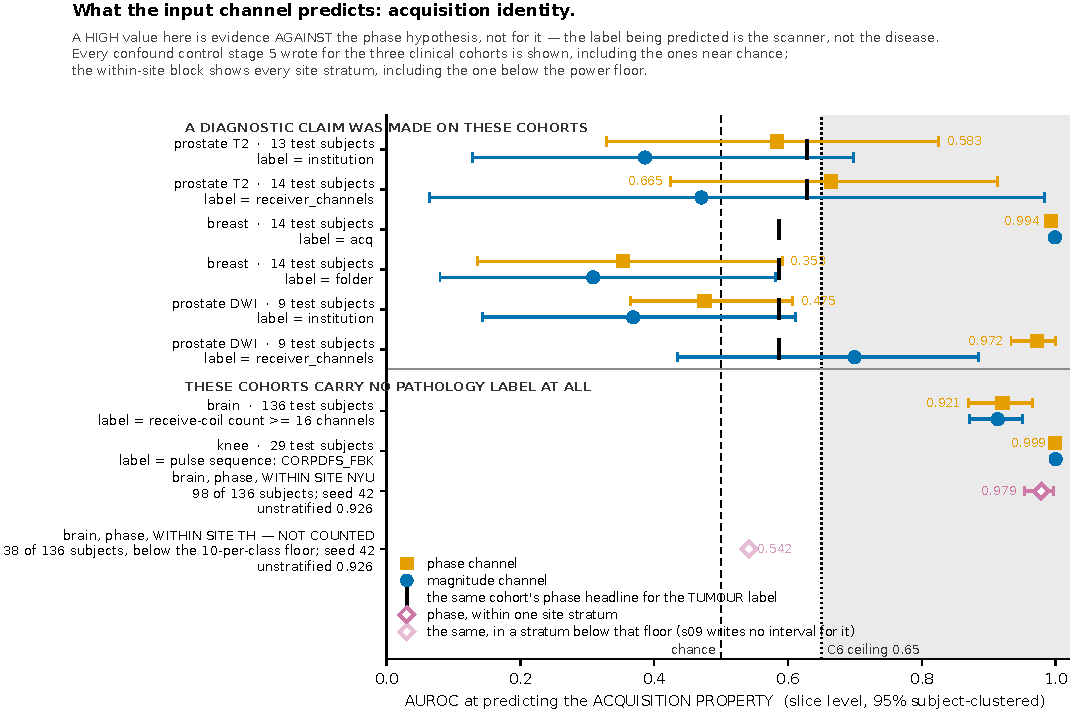
\includegraphics[width=\textwidth]{figures/figS1_acquisition_fingerprint.pdf}
\caption{\textbf{AUROC at predicting an acquisition property, not a diagnosis, from the
same input channels.} Slice-level AUROC with 95\% subject-clustered intervals.
\textbf{Upper block:} every \texttt{confound\_predictability} control stage 5 wrote for
the three cohorts on which a diagnostic claim was made --- prostate T2 and prostate DWI
against \texttt{institution} and \texttt{receiver\_channels}, breast against
\texttt{acq} and \texttt{folder} --- with the test-subject count printed beside each
row. All of them are shown, including the ones whose intervals cross chance; none was
selected on its value. Only the magnitude and phase arms appear, because stage 5 wrote
no \emph{both} arm for this control on these cohorts, and the gap is left empty rather
than filled. The black tick on each cohort's rows is that cohort's own phase headline
\emph{for the tumour label}, placed on the same axis so the two can be compared
directly. \textbf{Lower block:} the two cohorts whose label contains no pathology of
any kind --- brain, labelled by receive-coil count $\geq 16$ channels, and knee,
labelled by pulse sequence --- plus the brain phase arm recomputed inside each site
stratum, one row per stratum. The dotted line is the 0.65 ceiling written into criterion C6,
read here out of the criterion's own rule string;
the dashed line is chance. \textbf{A high value on this axis is evidence against the
phase hypothesis, because the label being predicted is the scanner and not the
disease.}
\textbf{Reading the within-site rows.} The brain cohort's 136 test subjects split
98/38 between two sites, and the estimate is carried by the 98-subject stratum:
it is the only one that clears the 10-per-class floor set before the analysis.
The 38-subject stratum has 6 subjects in one class, sits at 0.542, and is drawn
without an interval because \texttt{s09\_robustness.json} writes none for a
stratum below the floor. It is drawn rather than dropped: this figure claims to
show every control including the near-chance ones, and that has to include this
one. Both rows are the first of two seeds, which is stated on the rows; on the
second seed the same two strata give 0.974 and 0.578, so the qualitative reading
is stable across seeds and the point estimate is not a cohort-level within-site
figure. The 0.926 printed beside these rows as the unstratified comparator and the
0.921 on the brain row above are the same measurement read from two different
artefacts, \texttt{s09\_robustness.json} and \texttt{verdict.json}, which do not
aggregate the two seeds the same way: the per-seed unstratified values are 0.926
and 0.923, and \texttt{verdict.json}'s cohort figure is 0.921. The difference is
the aggregation and not a disagreement about the data, and both are shown rather
than one being quietly dropped. What the separability analysis in
\texttt{s09\_robustness.json} licenses is the scanner-and-coil configuration
taken together, tested in the only stratum where it can be tested: it is not
decomposable into coil count versus scanner model, and no such decomposition is
claimed. Sources: \texttt{pipeline\_out/report/verdict.json},
\texttt{pipeline\_out/robustness/s09\_robustness.json} and the per-cohort
\texttt{confound\_predictability} payloads under
\texttt{pipeline\_out/controls/results/}.}
\label{fig:confound}
\end{figure}

\subsection{Reconstruction fidelity, with its distribution and its floor}

Section~S4 reports the mean correlation against the vendor reference for each cohort.
A mean hides a distribution, and a correlation between two images of the same body part
is bounded away from zero by the shared body support alone. Figure~\ref{fig:reconfid}
shows both: the spread of the per-slice correlations, and the part of each that is
specific to the slice rather than to the anatomy.

\begin{figure}[htbp]
\centering
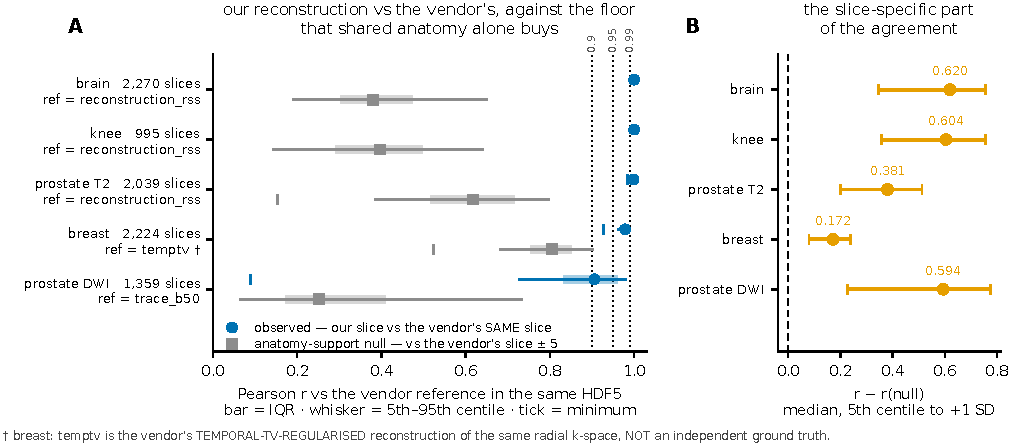
\includegraphics[width=\textwidth]{figures/figS2_recon_fidelity.pdf}
\caption{\textbf{Our reconstruction against the vendor reference shipped in the same
HDF5 file.} \textbf{(A)} Per-slice Pearson $r$ per cohort: the bar is the interquartile
range, the whisker the 5th to 95th centile, the tick the minimum, and the name of the
vendor reference dataset is printed beside each row together with the number of slices
the row actually plots --- that is, those with a computable correlation, which for
breast is 2{,}224 of the 2{,}240 cached and matches Table~\ref{tab:reconDetail} rather
than the cohort's cache size. Plotted
against each is the anatomy-support null --- the same slice of ours correlated with the
vendor's reference \emph{five slices away} in the same volume --- which is the floor
that shared anatomy buys before any reconstruction is correct. \textbf{(B)} The
difference, $r$ minus that floor, summarised by its median with the 5th centile to
$+1$~SD; Table~\ref{tab:anatomyfloor} gives the \emph{mean} of the same quantity, so
the two will not agree to the last digit and are not meant to. Breast is marked because
\texttt{temptv} is the vendor's temporal-TV-regularised reconstruction of the same
radial $k$-space rather than an independent ground truth, so its row is agreement
between two estimators; the prostate DWI per-slice row carries a deliberate SNR penalty
explained in Section~S4. Every vendor reference here is a magnitude image, so nothing
in this figure validates the phase channel. Sources:
\texttt{pipeline\_out/recon\_fidelity/recon\_fidelity\_summary.json} and the per-cohort
CSVs beside it.}
\label{fig:reconfid}
\end{figure}

\clearpage
\subsection{The estimator's input on the remaining four cohorts}

The main article shows all four columns --- magnitude, $\sin\varphi$, $\cos\varphi$
and the raw angle --- for the primary cohort.
Figure~\ref{fig:qualcohorts} shows the other four cohorts more briefly, on the same
selection rule: the magnitude channel and the raw angle only, because
$\sin\varphi$ and $\cos\varphi$ are a fixed pointwise function of that angle and
eight further panels of them would fill a page without adding one. It is included so
that a reader can see what a phase map looks like on a diffusion cohort, on a radial
breast acquisition and on the two hardware-labelled cohorts, rather than take the
description on trust.

% ---------------------------------------------------------------------------
% figures/figS3_qualitative_cohorts.pdf is NOT in the public git repository.
% It embeds fastMRI-derived MRI slices; the NYU fastMRI data sharing agreement
% permits use in an academic publication and forbids redistribution. It is
% named in paper/tex/.gitignore and is supplied to the journal out of band.
% make_figures.py rebuilds it from pipeline_out/cache/*.h5.
% ---------------------------------------------------------------------------
% width is 0.72 rather than 1.0 because this figure is nearly square and its
% caption carries the full per-panel provenance plus the breast label note; at
% \textwidth the float is taller than the page, and at 0.78 the last caption
% line runs into the folio.
\begin{figure}[p]
\centering
% Contains fastMRI image data; excluded from the public repository. See the
% corresponding note in main.tex.
\IfFileExists{figures/figS3_qualitative_cohorts.pdf}{%
  \includegraphics[width=0.72\textwidth]{figures/figS3_qualitative_cohorts.pdf}%
}{%
  \fbox{\parbox{0.88\textwidth}{\vspace{1em}\centering\small
  \textbf{Figure omitted from the public repository.}\\[0.4em]
  This panel displays NYU fastMRI image data, which the Data Sharing Agreement
  permits in an academic publication but not in a redistributable archive.
  Rebuild it from the licensed cache with
  \texttt{python paper/tex/make\_figures.py}.\vspace{1em}}}%
}
\caption{\textbf{The estimator's input on the four cohorts not shown in the main
article, one slice of each class.} For each cohort, columns 1--2 are the positive class
and columns 3--4 the negative class; within each pair, the first panel is the magnitude
channel as fed, per-slice z-scored, and the second is the raw phase in radians on a
cyclic scale. The raw angle is shown for orientation only and is never fed to any
estimator; what is fed is $\sin\varphi$ and $\cos\varphi$, computed from it. The cyan
outline is the stage-2 body mask. \textbf{(A)} prostate DWI: cache row 1279,
\texttt{file\_prostate\_AXDIFF\_052.h5}, slice 10, patient 52, tumour annotated;
against cache row 904, \texttt{file\_prostate\_AXDIFF\_038.h5}, slice 27, patient 38,
no tumour annotated. \textbf{(B)} breast: cache row 1888,
\texttt{fastMRI\_breast\_290\_1.h5}, slice 25, patient 290, label 1; against
cache row 1792, \texttt{fastMRI\_breast\_287\_1.h5}, slice 62, patient 287, label 0.
\textbf{The breast panels read ``label $=$ 1/0 (patient level)'' and not ``tumour
annotated on this slice'', because the breast label is not a slice annotation}: it
is the release's patient-level lesion status, 1 for malignancy with benign and
negative both mapped to 0, broadcast unchanged to all 32 cached slices of the
patient. No breast patient in the index carries more than one distinct slice label,
and nine patients in the negative class have a recorded benign lesion, patient 287
among them. The wording is set by a test on the index rather than by hand: a cohort
gets ``on this slice'' only where the index shows the label varying within a
patient, which it does for prostate T2 and DWI (31 of 67 and 24 of 45 patients) and
not for breast.
\textbf{(C)} brain: cache row 1160,
\texttt{file\_brain\_AXT2\_200\_6002484.h5}, slice 4, patient \texttt{brain\_0151},
label $\geq 16$; against cache row 1655,
\texttt{file\_brain\_AXT2\_207\_2070148.h5}, slice 4, patient \texttt{brain\_0239},
label $<16$. \textbf{(D)} knee: cache row 462, \texttt{file1001090.h5}, slice 18,
patient \texttt{knee\_0011}, label \texttt{CORPDFS\_FBK}; against cache row 522,
\texttt{file1001168.h5}, slice 14, patient \texttt{knee\_0094}, label
\texttt{CORPD\_FBK}. \textbf{The brain and knee labels are hardware and protocol
identity, not pathology} --- receive-coil count and pulse sequence --- and the class
names printed on the panels are stage 2's own \texttt{label\_name} values rather than
clinical terms. Every panel is drawn from the official test split by the rule used for
every qualitative panel in this work: the median row at that label, in cache order. No
panel was ranked on any outcome. The arrays are read from the stage-2 cache in stored
order, with no transpose, no re-reconstruction and no per-slice rescaling of phase.
\textbf{This figure illustrates the input and is not evidence for or against any
hypothesis}; the null rests on the intervals and the falsification suite, not on the
appearance of a slice. Data used in the preparation of this figure were obtained from
the NYU fastMRI Initiative database (\url{https://fastmri.med.nyu.edu}); see the data
source paragraph of Section~S4. Sources: \texttt{pipeline\_out/cache/*.h5}, their index
CSVs, and \texttt{pipeline\_out/report/verdict.json} for the class wording.}
\label{fig:qualcohorts}
\end{figure}

\end{document}
